%
% main.tex -- Paper zum Thema <wirbelringe>
%
% (c) 2020 Autor, OST Ostschweizer Fachhochschule
%
% !TEX root = ../../buch.tex
% !TEX encoding = UTF-8
% LTeX: enabled=false
\chapter{Wirbelringe\label{chapter:wirbelringe}}
\kopflinks{Wirbelringe}
\begin{refsection}
\chapterauthor{Nino Briker und Fabian Steiner}
\index{Nino Briker}%
\index{Briker, Nino}%
\index{Fabian Steiner}%
\index{Steiner, Fabian}%

%
% intro.tex -- Einleitung zum Thema
%
% !TEX root = ../../buch.tex
% !TEX encoding = UTF-8
%
\section{Einleitung}

Wirbelringe sind ein interessantes Naturphänomen welchem man schneller begegnet als man denkt. 
In diesem Paper schauen wir uns Wirbelringe etwas genauer an und begründen einige Eigenschaften. 
Des Weiteren untersuchen wir eine weitverbreitete praktische (ungewollte) Anwendung und dessen Auswirkung. 
Zuletzt formulieren wir ein Modell womit man zumindest angenähert selbst gezielt Wirbelringe berechnen und erzeugen kann.

In diesem Paper werden, wo nicht anders angegeben, nur ideale Fluide betrachtet.

\begin{quote}
    The theory of inviscid fluids is the study of «dry water».

    - John von Neumann \cite{Wirbelringe:feynman1964lectures}
\end{quote}

\subsection{Wirbel}

\begin{figure}
\centering
\begin{tikzpicture}
\clip (-6.3,-2.7) rectangle (6.3,2.7);
\node at (-0.07,-0.07) {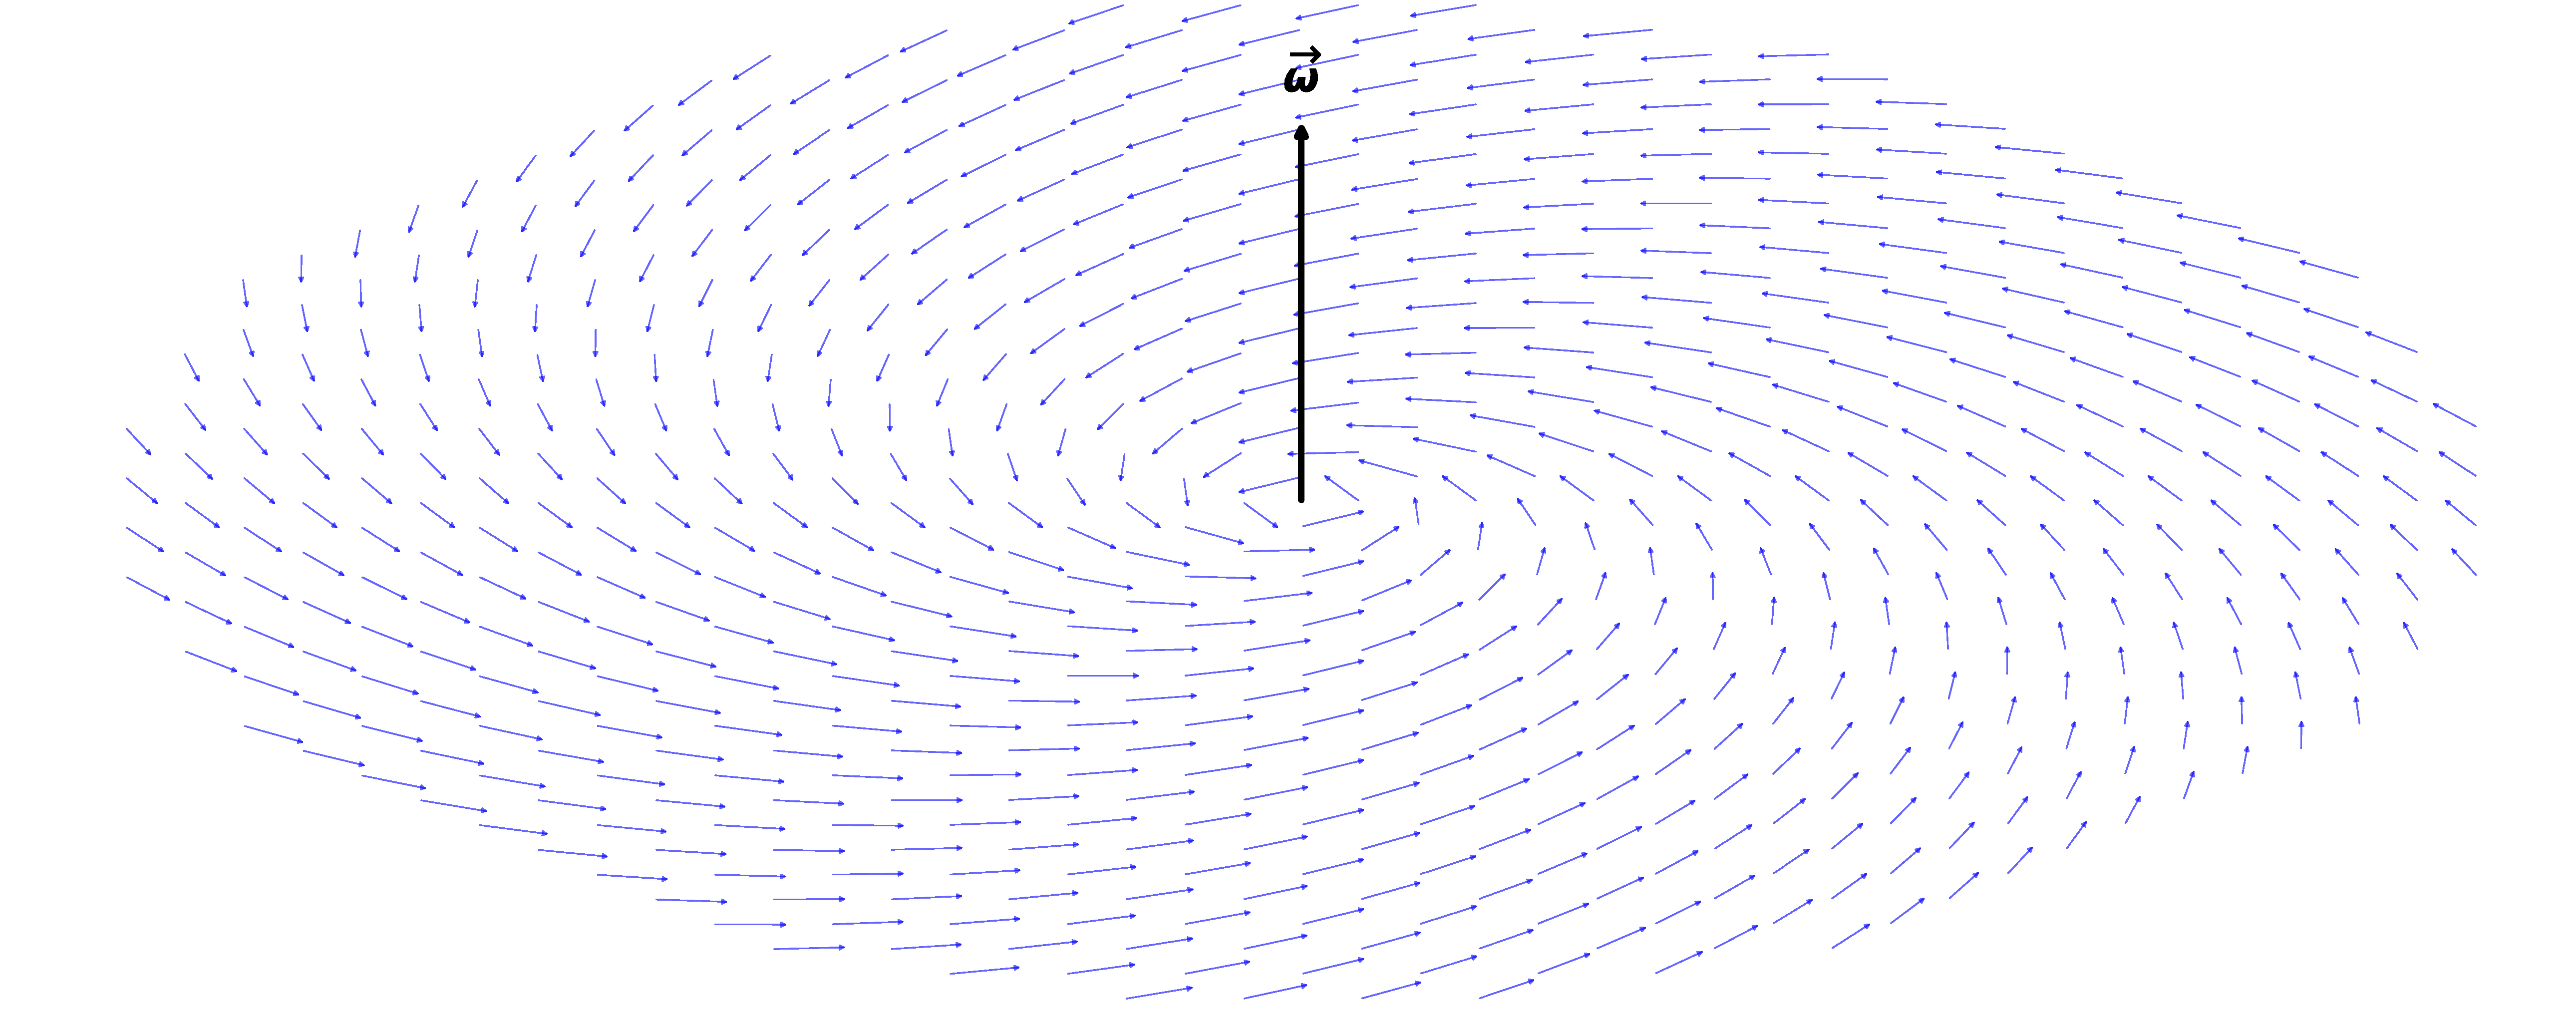
\includegraphics[width=1.08\textwidth]{papers/wirbelringe/fig/flacher_wirbel.pdf}};
%\draw[color=red] (-6.3,-2.7) rectangle (6.3,2.7);
\end{tikzpicture}
\caption{Darstellung eines 2-dimensionalen Wirbels mit Wirbelvektor
\(\vec{\omega}\).
\label{Wirbelringe:fig:flacher_wirbel}}
\end{figure}


Für die Betrachtung von Wirbelringen starten wir zunächst mit einzelnen Wirbeln.
Ein Wirbel ist eine Formation von Teilchen, welche um einen Mittelpunkt rotieren.
In Abbildung \ref{buch:papers:Wirbelringe:fig:flacher_wirbel} ist ein Wirbel abgebildet.
Die eingezeichneten Pfeile stellen die Geschwindigkeitsvektoren \( \vec{v} \) von den Teilchen dar, welche Teil des Wirbels sind.
Nicht explizit eingezeichnet sind die Bahnen, auf welchen sich die Teilchen bewegen.
Die Bahnen bilden konzentrische Kreise.
Auch ist in der Abbildung \ref{buch:papers:Wirbelringe:fig:flacher_wirbel} der Wirbelstärkevektor \(\vec{\omega}\) eingezeichnet.
Wir kommen später genauer auf \(\vec{\omega}\) zu sprechen.

\subsubsection*{Wirbellinien \label{paper:Wirbelringe:Wirbellinien}}

Um Wirbel besser zu beschreiben, führen wir hier den Begriff {\em Wirbellinie} ein.
Wirbellinien sind die „Mittelachsen“ eines Wirbels. 
Um diese Achse rotieren die Teile, welche Teil eines Wirbels sind. 
Diese hat an sich kein Volumen, allerdings kann es sein, dass Teilchen auf dieser Achse zu liegen kommen. 
\(\vec{\omega}\) steht tangential zu dieser Wirbellinie.  
In der Praxis ist eine Wirbellinie nicht gerade, sondern gekrümmt oder sogar spiralenähnlich. 
Des Weiteren ist eine sehr wichtige Eigenschaft, dass Wirbellinien nur auf einer Grenzfläche enden können, 
wie wir in Abschnitt \ref{paper:Wirbelringe:Grenzflaechen} sehen werden.

\subsection{Stabilität}

Um die Stabilität von Wirbeln zu beurteilen, können wir betrachten wie sich die Menge an Teilchen verhaltet, ob sie wächst oder schrumpft. 
Also die Divergenz der Teilchen, die Teil eines Wirbels sind.
Mit dieser Frage kommt man auf die Rechnung
\[
\operatorname{div} ( \operatorname{rot} ( \vec{A} ) )
= % \overset{!}{=}
?,
\]
wobei wir für \(\vec{A}\) das Vektorfeld aus Abbildung \ref{buch:papers:Wirbelringe:fig:flacher_wirbel} verwenden.
Nehmen wir an das \(\vec{A}\) zweimal stetig differenzierbar ist, so erhalten wir
\begin{align*}
\operatorname{div} ( \operatorname{rot} ( \vec{A} ) )
&=
\operatorname{div}      
    \begin{pmatrix} 
        \frac{\partial A_z}{\partial y} - \frac{\partial A_y}{\partial z} \\ 
        \frac{\partial A_x}{\partial z} - \frac{\partial A_z}{\partial x} \\ 
        \frac{\partial A_y}{\partial x} - \frac{\partial A_x}{\partial y} \\ 
    \end{pmatrix} \\
&=
\frac{\partial^2 A_z}{\partial x \partial y} - \frac{\partial^2 A_y}{\partial x \partial z} + 
\frac{\partial^2 A_x}{\partial y \partial z} - \frac{\partial^2 A_z}{\partial y \partial x} +
\frac{\partial^2 A_y}{\partial z \partial x} - \frac{\partial^2 A_x}{\partial z \partial y}
\\
&=
\frac{\partial^2 A_z}{\partial x \partial y} - \frac{\partial^2 A_z}{\partial y \partial x} + 
\frac{\partial^2 A_x}{\partial y \partial z} - \frac{\partial^2 A_x}{\partial z \partial y} +
\frac{\partial^2 A_y}{\partial z \partial x} - \frac{\partial^2 A_y}{\partial x \partial z}
\quad \text{(Satz von Schwarz)}\\
&=
\overbrace{\frac{\partial^2 A_z}{\partial x \partial y} - \frac{\partial^2 A_z}{\partial x \partial y}}^0 + 
\overbrace{\frac{\partial^2 A_x}{\partial y \partial z} - \frac{\partial^2 A_x}{\partial y \partial z}}^0 +
\overbrace{\frac{\partial^2 A_y}{\partial x \partial z} - \frac{\partial^2 A_y}{\partial x \partial z}}^0
\\
&=
0
\end{align*}

Aus dem Resultat
\begin{equation}
    \label{paper:Wirbelringe:eq:wIdent}
\operatorname{div} ( \operatorname{rot} ( \vec{A} ) ) 
= 
0
\end{equation}
lässt sich schliessen, dass Teilchen in einem Rotationsfeld erhalten bleiben. 
Das bedeutet, dass sie immer weiter rotieren. 
Aus diesem Grund sind Wirbel sehr Stabil.

\subsection{Vom Wirbel zum Wirbelring}

Um aus Wirbel ein Wirbelring zu machen brauchen wir noch eine Definition.

\subsubsection*{Wirbelfäden}

Ein {\em Wirbelfaden} ist ein Zylinder, welcher eine Wirbellinie als Zentrum des Zylinders hat.
Schneidet man nun diesen Zylinder senkrecht zu der Wirbellinie, ergibt sich ein einzelner Wirbel.
Wirbelfäden werden auch {\em Wirbelröhren} genannt.

Um aus einem Wirbelfaden ein Wirbelring zu machen, schliessen wir die offenen enden (wir betrachten später, wie man mit diesen umzugehen hat) zusammen.
Die Wirbellinie formt ein Kreis.
Jetzt ist es ein Wirbelring. 
Solch ein Wirbelring ist in Abbildung \ref{buch:papers:Wirbelringe:fig:generell} dargestellt.

\begin{figure}
\centering
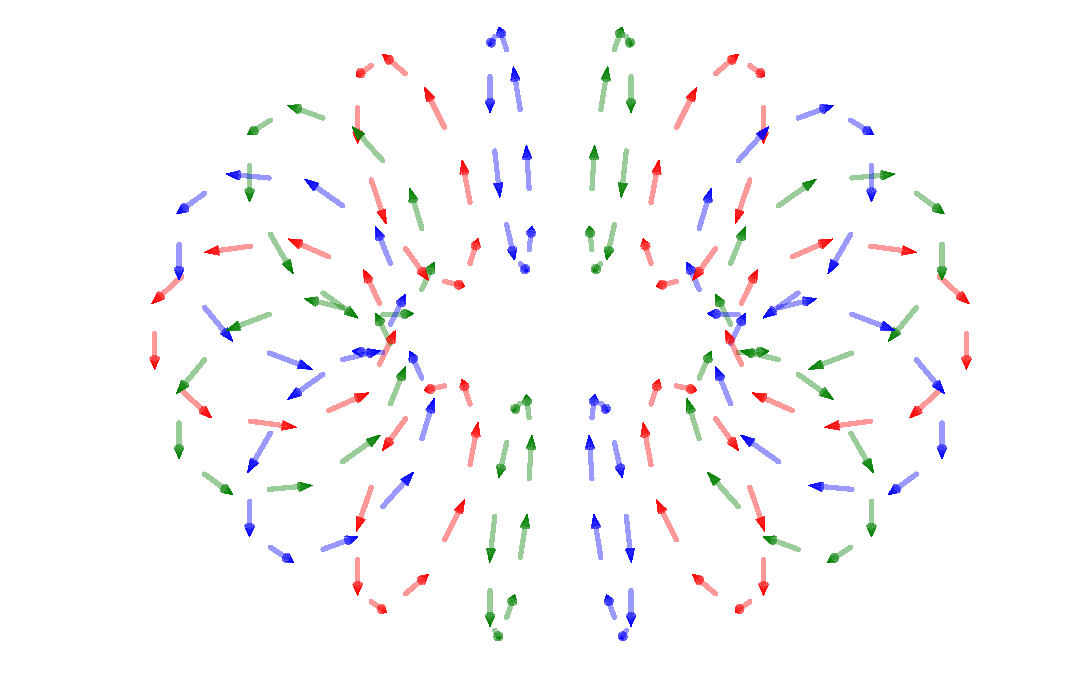
\includegraphics[width=1\textwidth]{papers/wirbelringe/fig/wirbelring_RGB.pdf}
\caption{Typischer idealer Wirbelring.
Dargestellt durch momentane Bewegungsvektoren unterschiedlicher Teilchen in regelmässigem Abstand.
Zur besseren Übersicht sind Teilchen eines Wirbels mit derselben Farbe markiert.
Unterschiedliche, benachbarte Wirbel haben unterschiedliche Farben.
Die Wirbellinie ist als schwarze, gestrichelte Linie eingezeichnet.\label{Wirbelringe:fig:generell}}
\end{figure}

\section{Helmholzsche Wirbelsätze}

\subsection{Historisches}

Um das Verhalten von Wirbelringen besser zu verstehen, sind die sogenannten helmholzschen Wirbelsätze sehr nützlich. 
Mitte 19. Jahrhundert formulierte der Deutsche Physiker Hermann von Helmholtz 3 Wirbelsätze und veröffentlichte diese im Journal für die reine und angewandte Mathematik\cite{Wirbelringe:JournalHelmholz}.
In dieser definiert er auch gleich auch Hilfslinien, um die Wirbelbewegungen, besser beschreiben zu können:

\subsubsection*{Wirbellinien}

Wirbellinien sind die „Mittelachse“ eines Wirbels. 
Um diese Achse rotieren die Teile, welche teil eines Wirbels sind. 
Diese hat an sich kein Volumen, allerdings kann es sein das Teilchen auf dieser Achse zu liegen kommen. 

\subsubsection*{Wirbelfäden}



\subsection{Erster Helmholzscher Wirbelsatz}

\begin{displayquote}
    In Abwesenheit von wirbel anfachenden äusseren Kräften bleiben wirbelfreie Strömungsgebiete wirbelfrei.
\end{displayquote}

Teilchen die, ruhen bleiben in ruhe.

\begin{figure}
\centering
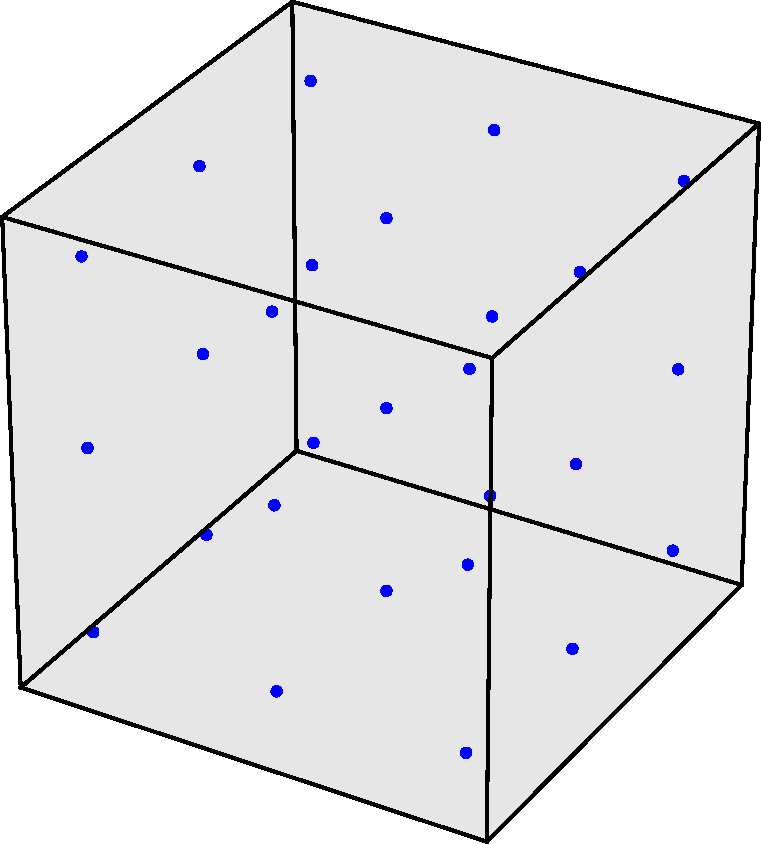
\includegraphics[width=0.4\textwidth]{papers/wirbelringe/fig/cube_still_particles.pdf}
\caption{Visuelle Darstellung des 1. helmholtzschen Wirbelsatz \label{buch:papers:Wirbelringe:fig:Helmholtz_1}}
\end{figure}

\subsection{Zweiter Helmholzscher Wirbelsatz}

\begin{displayquote}
    Fluidelemente, die auf einer Wirbellinie liegen, verbleiben auf dieser Wirbellinie.
\end{displayquote}

\begin{figure}
\centering
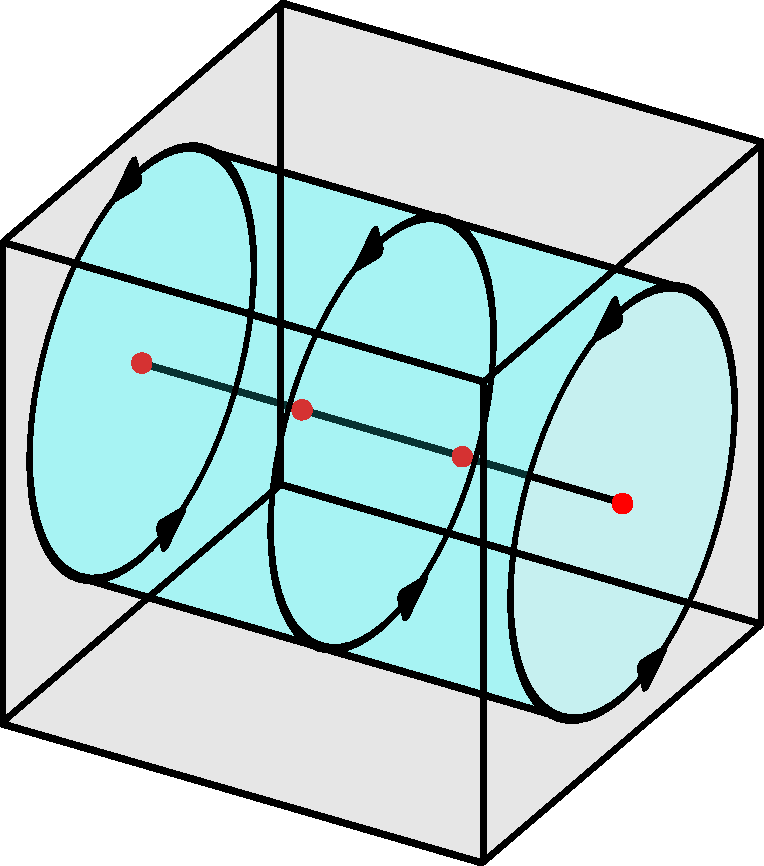
\includegraphics[width=0.4\textwidth]{papers/wirbelringe/fig/cube_still_particles_rotation.pdf}
\caption{Visuelle Darstellung des 2. helmholtzschen Wirbelsatz \label{buch:papers:Wirbelringe:fig:Helmholtz_2}}
\end{figure}

\subsection{Dritter Helmholzscher Wirbelsatz}

\begin{displayquote}
    Fluidelemente, die auf einer Wirbellinie liegen, verbleiben auf dieser Wirbellinie.
\end{displayquote}

\begin{figure}
\centering
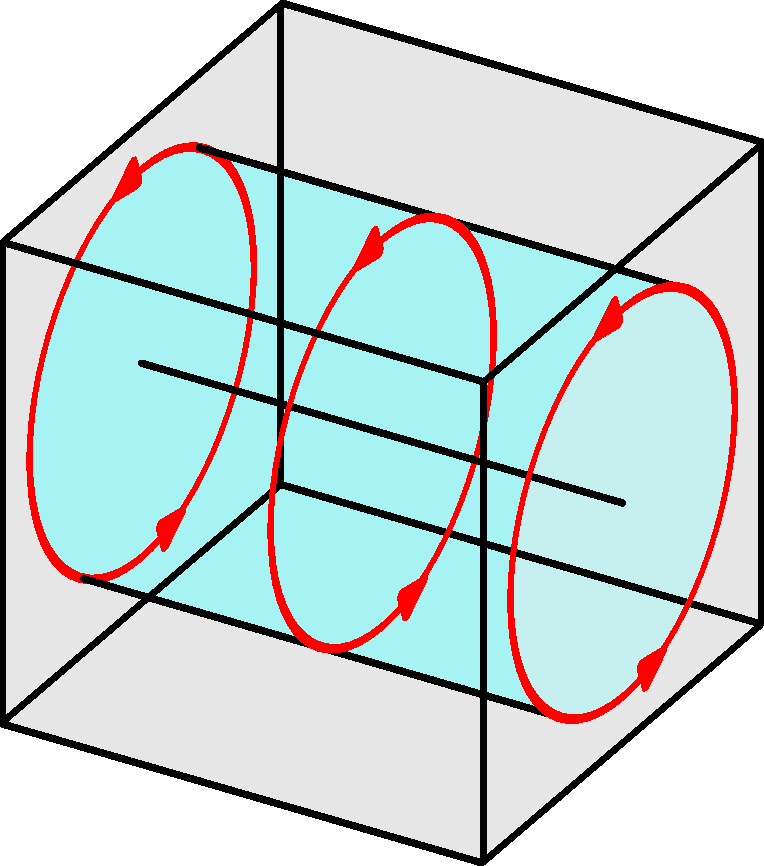
\includegraphics[width=0.4\textwidth]{papers/wirbelringe/fig/cube_constant_rotation.pdf}
\caption{Visuelle Darstellung des 3. helmholtzschen Wirbelsatz \label{buch:papers:Wirbelringe:fig:Helmholtz_3}}
\end{figure}

\subsection{Verhalten an Grenzflächen}
%
% bewegung.tex -- Begründet die Bewegung von Wirbelringen
%
% !TEX root = ../../buch.tex
% !TEX encoding = UTF-8
%
\section{Bewegung eines Wirbelrings\label{Wirbelringe:Bewegung}}

Bisher wurde die Bewegung eines Wirbelrings noch nicht weiter betrachtet. 
Doch wie man bereits bei Rauchringen beobachten kann, bleiben diese nicht an einem Ort stehen, sondern bewegen sich. 
Um diese Verhalten zu begründen, kann das Biot-Savart-Gesetz \cite{Wirbelringe:FuehrerdurchdieStroemungslehre} angewendet werden, was im folgenden Abschnitt gemacht werden soll.

\subsection{Biot-Savart-Gesetz}

Das Biot-Savart-Gesetz
\[
d \vec{B}
=
\frac{\mu_0}{4\pi}\frac{I \,d \vec{l} \times \vec{r}}{\left\lvert \vec{r}^{\,3}\right\rvert }
\]  % Note : diese Definition weicht von der Definiton 3.2 im ELT2 Skript ab da dort ein Richtungsvektor verwendet wird -> ein r (dort ein R) kürzt sich heraus
wird typischerweise in der Elektrotechnik angewendet, um das Magnetfeld von bewegten Ladungen zu beschreiben (hier nur auf einen Strom durch einen Leiter vereinfacht).
Es kann nur bei geschlossenen Stromkreisen verwendet werden. 

Damit wir das Gesetz nutzen können, müssen wir zunächst die Grössen anpassen und überprüfen, ob das überhaupt erlaubt ist. 
Die elektrodynamischen Grössen haben jeweils ein Gegenstück in der Strömungsmechanik:

\begin{center}
    \begin{tabular}{lcl}
    stromdurchflossener Leiter          & \(\Leftrightarrow \) & Wirbelfaden \\
    Stromstärke \(I\)                   & \(\Leftrightarrow \) & Zirkulation \(\Gamma\) \\
    Stromdichtevektor \(\hat{j}\)       & \(\Leftrightarrow \) & Wirbelstärkevektor \(\vec{\omega}\)\\
    magnetische Feldstärke \(\vec{H}\)  & \(\Leftrightarrow \) & Geschwindigkeit \(\vec{u}\) \\
    \end{tabular}
\end{center}

Im Folgenden wird der Wirbelstärkevektor nicht verwenden.
Jedoch ist der Zusammenhang vom Wirbelstärkevektor zum Stromdichtevektor etwas intuitiver als die Zirkulation zur Stromstärke.

Die Maxwellgleichungen (siehe Abschnitt \ref{chapter:maxwell}) sehen vor das \(\vec{B}\) Feld quellenfrei ist. 
Da wir nur inkompressible Fluide betrachten, ist dies gegeben.

Setzt man nun die entsprechenden Grössen in das Biot-Savart-Gesetz
\[
d\, \vec{u}
=
\frac{\Gamma}{4\pi}\frac{d\, \vec{l} \times \vec{r}}{\left\lvert \vec{r}^{\,3}\right\rvert }
\]
ein, lässt sich damit die Geschwindigkeitsänderung eines Punktes durch ein Wirbelfadenelement beschreiben.
Um die Rechnung zu vereinfachen, können wir annehmen, dass der Wirbelfaden vergleichsweise dünn ist, verglichen zum Durchmesser des Rings aus der Wirbellinie.
Mit dem Integral über diesen Wirbelfaden
\[
\vec{u}
=
\int_{\text{Wirbellinie}} \frac{\Gamma}{4\pi}\frac{d\, \vec{l} \times \vec{r}}{\left\lvert \vec{r}^{\,3}\right\rvert}
\]
erhalten wir die induzierte Geschwindigkeit, welche durch den Wirbelfaden entsteht.
Da dieses Gesetz aus der Elektrotechnik stammt, spricht man in der Strömungsmechanik von einer induzierten Geschwindigkeit.

Um nun die selbstinduzierte Geschwindigkeit zu berechnen, wählen wir ein in der X-Y Plane liegender Wirbelring mit Radius \(a\).
Der Radius des Wirbelfaden ist einfachheitshalber verglichen zum Radius der Wirbellinie vernachlässigbar klein.
Uns interessiert irgendein Punkt, der auf der Wirbellinie liegt.
Somit ist
\(
\vec{r} = 
\begin{pmatrix}
    a\\
    0\\
    0    
\end{pmatrix}\)
und
\(
d\,\vec{l} = 
\begin{pmatrix}
    0\\
    a\\
    0    
\end{pmatrix}d\,\varphi \). 
Setzt man diese in
\[
\vec{u}
=
\int_{0}^{2\pi} \frac{\Gamma }{4\pi}\frac{d\, \vec{l} \times \vec{r}}{\left\lvert \vec{r}^{\,3}\right\rvert },
\]
ein erhält man 
\[
\vec{u}
=
\frac{\Gamma a^{2}}{4\pi a^{3}} \int_{0}^{2\pi} \hat{z}\, d\,\varphi.
\]
Da der Kreisumfang und der Radius immer senkrecht zueinander ist der Richtungsvektor \(\hat{z}\). 
Schlussendlich ergibt sich
\[
\vec{u}
=
\frac{\Gamma }{2 a}\hat{z},
\]
woraus ersichtlich ist das, je kleiner der Wirbelring, desto schneller bewegt er sich.

Würde man dieselbe Rechnung für einen geraden Wirbelfaden durchführen, würde auffallen, dass das Ergebnis für Punkte auf der Wirbellinie null ist.
Der Wirbelfaden induziert sich selbst keine Geschwindigkeit.
Daher, damit sich ein Wirbelfaden von sich bewegt, muss dieser zumindest ein wenig gekrümmt sein.
Ein zweiter Wirbelfaden würde zu einer induzierten Geschwindigkeit führen. 
Dies betrachten wir hier aber nicht weiter. 

\subsection{Bewegung eines Teilchens}

\begin{figure}
\centering
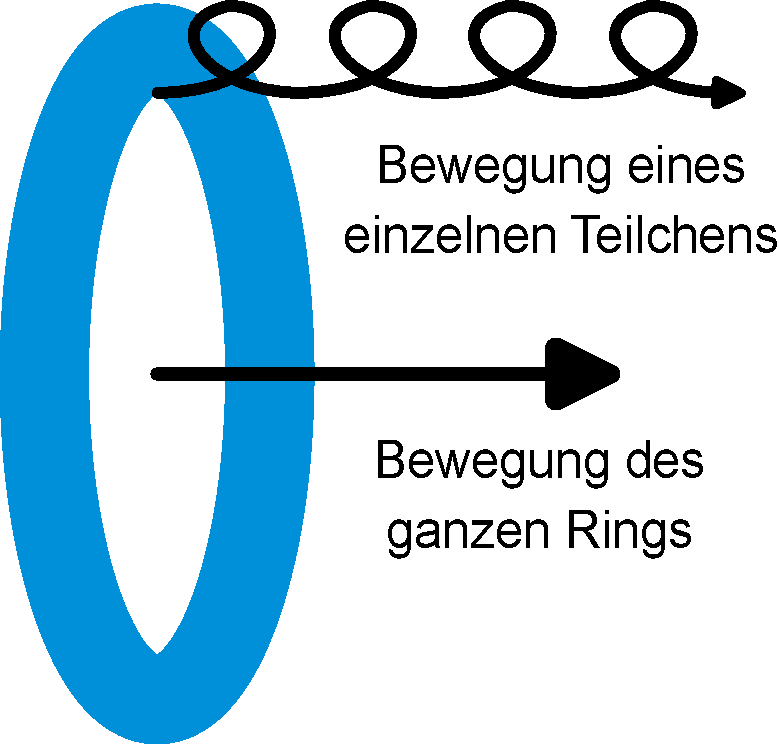
\includegraphics[width=0.4\textwidth]{papers/wirbelringe/fig/ausbreitung_teilchen.pdf}
\caption{Bewegung eines einzelnen Teilchen ToDo besseri Farb für de Ring??? \label{buch:papers:Wirbelringe:fig:ausbreitung_teilchen}}
\end{figure}

Eine interessante Kurve zeichnet sich ab, wenn man ein einzelnes Teilchen beobachtet.
Es bildet sich eine Zykloide.
Die Grösse der Zykloide hängt von der Höhe der Zirkulation ab.
Dies ist in Abbildung \ref{Wirbelringe:fig:ausbreitung_teilchen} dargestellt.

%
% Wirbelschleppe.tex -- Erleutert Wirbelschleppen
%
% !TEX root = ../../buch.tex
% !TEX encoding = UTF-8
%
\section{Wirbelschleppe}
An einem nebligen Tag kann man sie an einem Flughafen gut beobachten. 
Die Rede ist von den Wirbelschleppen hinter den Enden der Tragflächen eines Flugzeugs.
Aber wieso entstehen sie eigentlich? 
Wo genau starten sie und wo ist deren Ende?
Wieso schaudert es Kleinflugzeug-Piloten, wenn sie diesen Begriff hören?
All das und mehr klären wir in diesem Abschnitt mit ein wenig Mathematik.
\begin{figure}
\centering
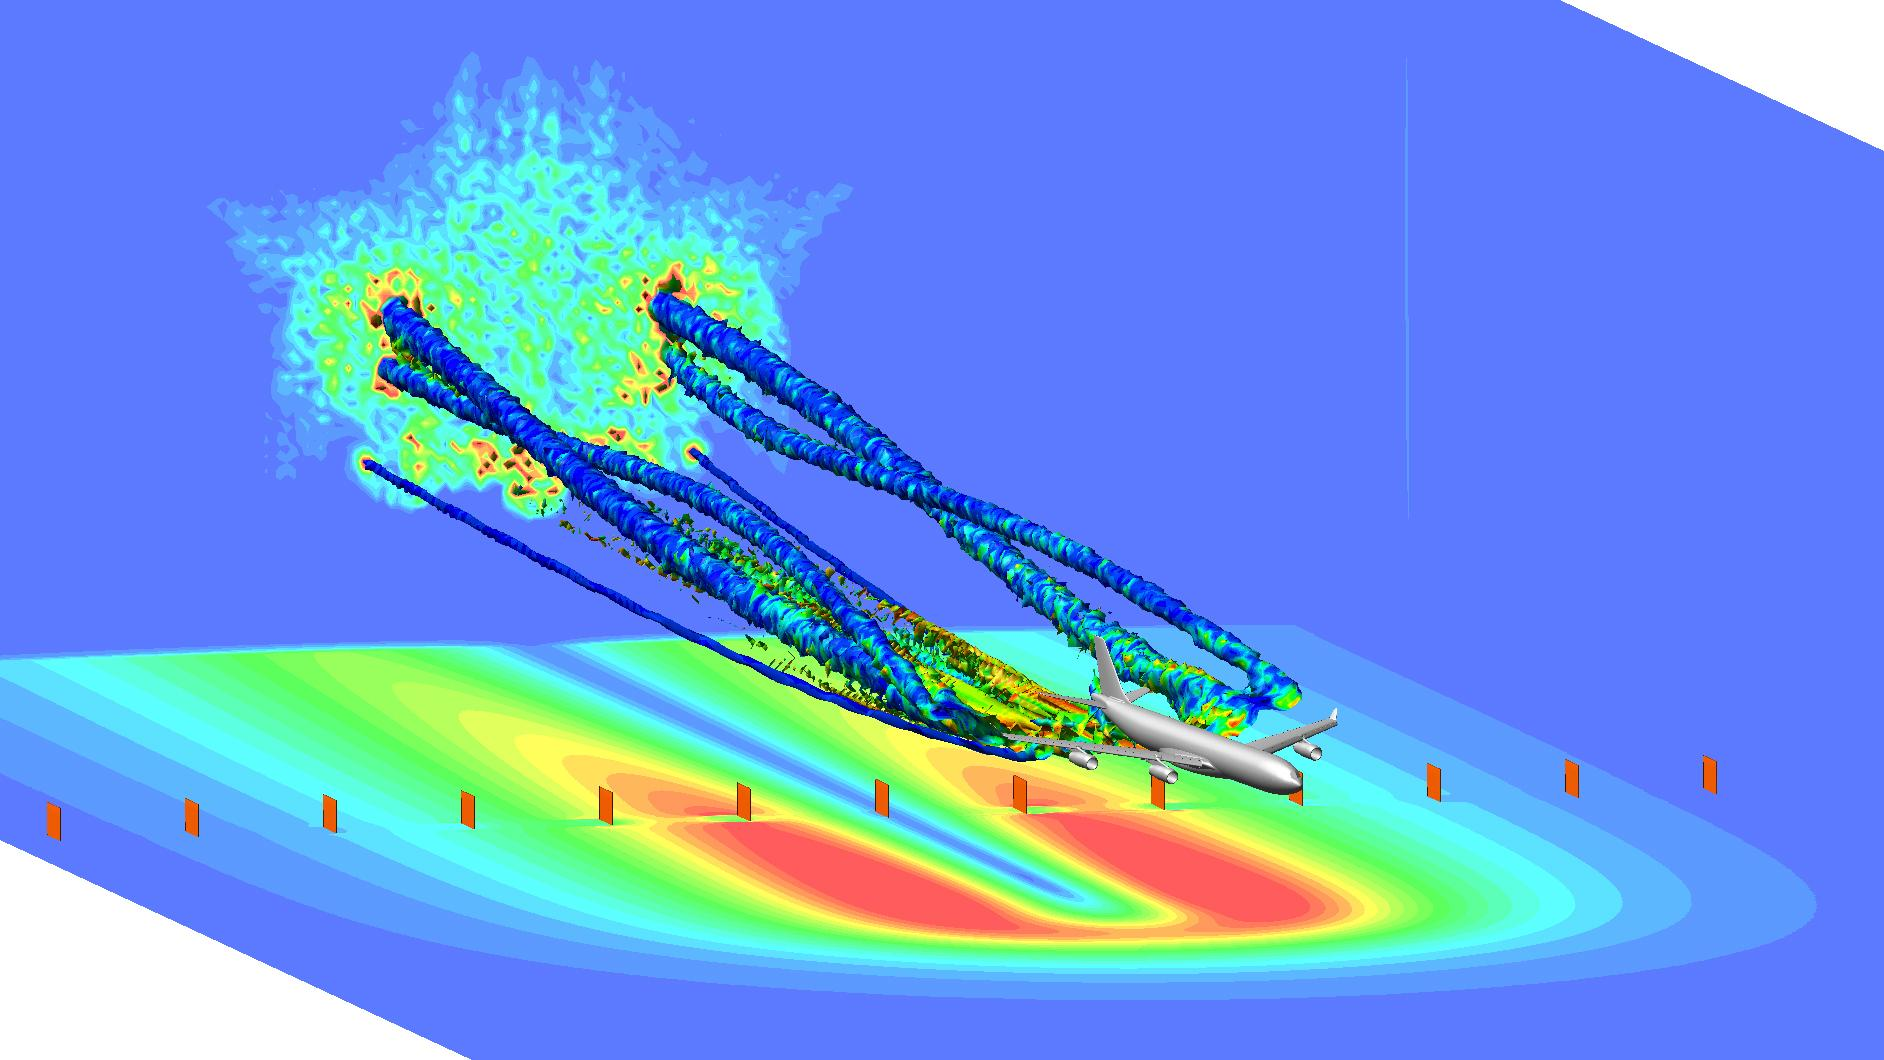
\includegraphics[width=0.8\textwidth]{papers/wirbelringe/fig/wirbelschleppen_in_der_simulation.jpg}
\caption{Simulation der Wirbelschleppenbildung eines Airbus A340 im Endanflug kurz vor der Landebahn
\cite{Wirbelringe:wirbelschleppen_in_der_simulation}. \label{Wirbelringe:fig:wirbelschleppen_in_der_simulation}}
\end{figure}

\subsection{Entstehung}
Wirbelschleppen bilden sich genau am Ende der Tragfläche aufgrund des Druckunterschieds, welcher das Flugzeug in erster Linie Fliegen lässt.
Um deren Entstehung genauer anschauen zu können gibt es nun einen kleinen Theorieausschnitt aus der Aviatik:
Setzt sich ein Flugzeug in Bewegung, so entsteht um die Flügeltragflächen ein Luftstrom.
Ein weitverbreiteter Irrglaube besagt, dass die Luft, welche über den Flügel geht, \glqq länger\grqq hat und deshalb schneller sein muss.
Dies ist jedoch nicht ganz korrekt.
Es ist vielmehr die \textbf{Fläche} eines einzelnen, gedachten Luftstroms, welche auf dem Flügel verkleinert wird.% TODO: Genauere Erklärung noch anfügen!
Wenn man dann mittels Kontinuitätsgleichung

\[
v_{\text{oben}}A_{\text{oben}} 
=
v_{\text{unten}}A_{\text{unten}}
\]
die Geschwindigkeiten der beiden gedachten Luftströme vergleicht, muss der Luftstrom mit Geschwindigkeit $v_{\text{oben}}$ schneller sein als $v_{\text{unten}}$.
Dies hat jetzt zur Folge, dass laut dem Satz von Bernoulli 
\begin{equation}
    p+\frac{1}{2}\rho v^2+\rho gh
    =
    const
    \label{paper:Wirbelringe:eq:Bernoulli}
\end{equation}

der Druck $p_{\text{oben}}$ kleiner sein muss als der Druck $p_{\text{oben}}$.
Nimmt man jetzt jeweils einen Punkt auf der Ober- sowie einen auf der Unterseite und setzen diese in \ref{paper:Wirbelringe:eq:Bernoulli} ein, so können sie 
\[
p_{\text{oben}}+\frac{1}{2}\rho v^2_{\text{oben}} + \rho gh_1 
=
p_{\text{unten}}+\frac{1}{2}\rho v^2_{\text{unten}}+\rho gh_2
\]
gleichgesetzt werden.
Jetzt kann angenommen werden, dass der Höhenunterschied zwischen den beiden Punkten ober und unterhalb des Flügels vernachlässigbar klein ist also \(h_1\approx h_2\).
Zudem ist die Dichte der Luft an beiden Punkten ungefähr gleich, weshalb sich der Term zu 
\[
p_{\text{oben}}+\frac{1}{2}\rho v^2_{\text{oben}} 
=
p_{\text{unten}}+\frac{1}{2}\rho v^2_{\text{unten}}
\]
vereinfacht.
Für die Druckdifferenz ergibt sich
\[
p_{\text{oben}}-p_{\text{unten}} 
=
\frac{1}{2}\rho( v^2_{\text{unten}}-v^2_{\text{oben}})
\]
und man kann erkennen, dass wenn $v_{\text{unten}} < v_{\text{oben}}$ muss $p_{\text{unten}} > p_{\text{oben}}$ sein.

Mit diesem Wissen kann auch die Entstehung der Wirbelschleppe erklärt werden. 
Es existiert also unterhalb des Flügels ein Überdruck und oberhalb ein Unterdruck.
Solange ein Flügel dazwischen ist, generiert dieser Druckunterschied einen Auftrieb, was gut und auch gewünscht ist.
Dummerweise gibt es aber eine Stelle, an der der Flügel endet und dort wirds dann auch spannend.
An der Spitze des Flügels findet nämlich ein Druckausgleich statt.
Hierbei strömt die Luft unterhalb des Flügels nach oben in das Unterdruckgebiet. 
Dabei entsteht eine Zirkulation $\Gamma$, sie zirkuliert um den ganzen Flügel.
Schlussendlich wird sie zu einer Wirbelschleppe am Flügelende.
Die entstandene Wirbelschleppe hat ein paar interessante Eigenschaften, welche in den kommenden Abschnitten behandelt werden.

\subsection{Wirbellinie}
Wie bereits im Kapitel \ref{paper:Wirbelringe:Wirbellinien} erwähnt sind Wirbellinien immer geschlossen oder enden auf Grenzflächen.
Die Wirbelschleppe jedoch hat eine ganz spezielle Wirbellinie, da diese eine Gerade von dem Flügelende bis zum Ort an dem das Flugzeug gestartet ist.
Dies klingt zunächst etwas seltsam und unglaubwürdig und natürlich ist diese Aussage auch nicht ganz korrekt.
Denn in der Realität wird sich die Wirbelschleppe natürlich irgendwann aufgrund des Luftwiderstands auflösen und somit auch die Wirbellinie verschwinden.
Also gibt es leider oder eben zum Glück keine Wirbelschleppe von Zürich nach Tokyo, wenn man mit dem Flugzeug etwaige Enkel besuchen geht.
Aber die Bedingung ist auch hier erfüllt, da die Wirbellinie am Flügelende (Grenzfläche zwischen Luft und Aluminium) startet und am Boden des Flughafens (Grenzfläche zwischen Asphalt und Luft) endet.

\begin{figure}
\centering
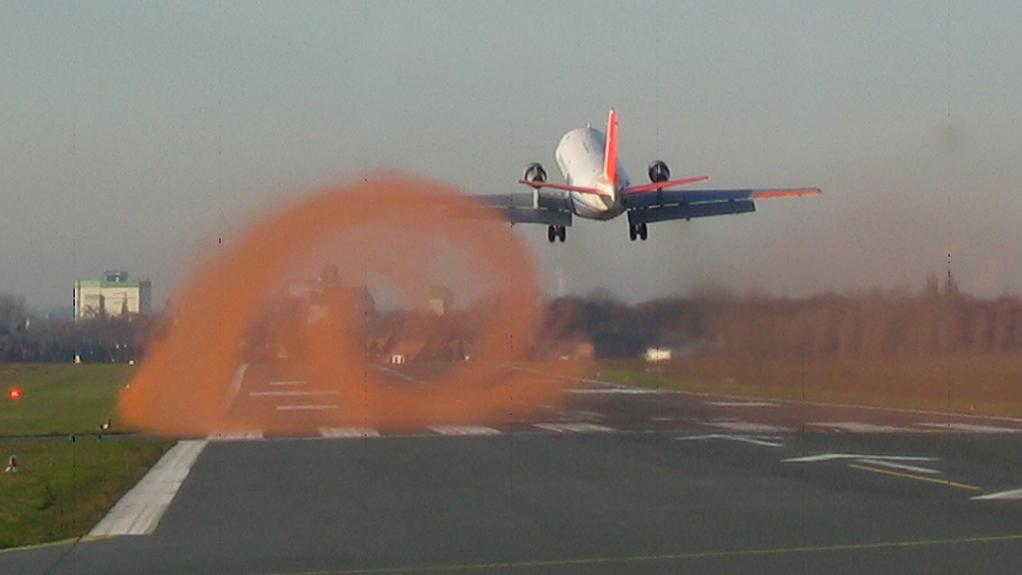
\includegraphics[width=0.8\textwidth]{papers/wirbelringe/fig/visualisierung_einer_wirbelschleppe.jpg}
\caption{Sichtbar gemachte Wirbelschleppe 
\cite{Wirbelringe:visualisierung_einer_wirbelschleppe} \label{buch:papers:Wirbelringe:fig:visualisierung_einer_wirbelschleppe}}
\end{figure}

\subsection{Problematik in der Aviatik}
Da Wirbelringe sehr stabil sind und sich nicht sofort auflösen, bleiben auch die Wirbelschleppen relativ lange bestehen.
Zudem breiten sie sich seitlich aus und sinken hinter dem Flugzeug ab.
Bei \glqq schweren\grqq Flugzeugen (ab 136 Tonnen MCTOW\footnote{maximum certified takeoff weight oder zu Deutsch: maximales Startgewicht}) \cite{Wirbelringe:WakeTurbulence} wird vorgeschrieben, dass nachfolgende Flugzeuge bis zu 3 Minuten warten müssen bevor sie starten dürfen.
Denn sollte ein Kleinflugzeug kurz nach einem solchen Flugzeug starten wird es ziemlich sicher von dessen Wirbelschleppe erfasst.
In ganz schlimmen fällen kann dies durchaus zu einem Absturz führen.
Ebenfalls muss man bedenken, dass es Energie benötigt eine solche Wirbelschleppe aufrechtzuerhalten.
Die Energie dafür wird natürlich aus den Triebwerken des Fliegers gewonnen, welcher aber eigentlich dafür gedacht war, Passagiere von A nach B zu bringen.
Deshalb finden die Airlines es grundsätzlich nicht sehr amüsant, zwei gewaltige Wirbelschleppen hinter ihren Flugzeugen herzuziehen, auch wenn es bei Schlechtwetter sehr spektakulär aussehen kann (siehe \ref{wirbelringe:fig:Wirbelschleppe}). %TODO: Gschiids bild finde
Findige Wissenschaftler waren deshalb auf die Idee der Winglets gestossen.
Diese sollten durch Reduktion der Zirkulation an den Flügelenden die Bildung solcher Wirbelschleppen hemmen.
Bei diesem unterfangen hatten sie auch Erfolg aber zu einem preis, welcher in der Aviatik nicht gern gesehen ist.
Durch das Anbringen solcher Winglets an den Flügelenden steigt das Leergewicht des Flugzeuges an.
Das bedeutet, dass dieses zusätzliche Gewicht wieder mehr Treibstoff verbraucht.
Wieso werden diese aber trotzdem in Kurzstreckenflugzeugen eingesetzt?
Einerseits haben Winglets zusätzlich die angenehme Eigenschaft, den Lärm eines Flugzeuges zu reduzieren.
Andererseits höhlt bekanntlich steter Tropfen den Stein.
Wenn ein Kurzstreckenflieger täglich 5-6 mal fliegt und dabei jedes Mal 1-2 \% Treibstoff spart, so summiert sich dies und wird wieder Lohnenswert für die Fluggesellschaften.
Bei Langstreckenflügen hingegen lohnen sich die Winglets noch viel mehr, da bei längerem Flug auf Reiseflughöhe (\textasciitilde10'000 m.ü.M.) auch die Wirkung der Winglets länger genutzt werden kann.

%
% slugModell.tex -- Erleutert das Slug Modell
%
% !TEX root = ../../buch.tex
% !TEX encoding = UTF-8
%
\section{Slug Modell}
In diesem Kapitel werden wir uns das Slug Modell etwas genauer unter die Lupe nehmen, um die Entstehung eines Wirbelrings etwas genauer zu verstehen.
Die genaue mathematische Beschreibung des Entstehungsprozesses ist sehr komplex und würde den Rahmen dieses Kapitels sprengen.
Dafür kann mittels Slug Modell dieser Prozess relativ genau angenähert werden.

\subsection{Grundlegende Idee}
Im Slug Modell wird der Impulsaustritt eines Fluidvolumens (eines Fluid-Slug) aus einer Öffnung beschrieben.
Man kann sich dies als Zylinder aus Flüssigkeit vorstellen, welcher innert kürzester Zeit aus einer Öffnung geschoben wird.
Dabei definieren wir folgende Grössen:
\begin{itemize}
    \item Zirkulation $\Gamma$
    \item Wirbelstärke $\omega$
    \item Slug Geschwindigkeit $u_p(t)$
    \item Slug Durchmesser $D$
    \item Slug Länge $L$
\end{itemize}
Tritt nun das Slug aus dem Zylinder aus, so trifft die Aussenseite des Slugs auf das stehende Fluid (bspw. Luft oder Wasser) ausserhalb.
Dies bewirkt aufgrund der Geschwindigkeitsdifferenz zwischen dem Inneren des Slugs und dem stehenden Fluid aussen eine Scherung.
Die Scherung hat zur Folge, dass sich das Slug beginnt \glqq Aufzurollen\grqq und somit einen Wirbel formt. 
Die in Abschnitt \ref{paper:Wirbelringe:Stokes} genannten Formel für die Zirkulation kann approximativ auf
\[
\Gamma \approx \frac{1}{2}UL
\]
vereinfacht werden.


%
% WirbelringKanone.tex -- praktische Aplikation und anleitung zum Bau einer Wirbelringkanone
%
% !TEX root = ../../buch.tex
% !TEX encoding = UTF-8
%
\section{Praktische Applikation und Versuch für zu Hause}

Im Zuge der dieser Seminararbeit wurden unsere Erkenntnisse an einer Präsentation vorgestellt. 
Dieses Thema bietet eine interessante Möglichkeit es zu visualisieren. 
Dies ist eine Wirbelringkanone. 
Damit lassen sich gezielt Wirbelringe erzeugen, um damit die Eigenschaften davon zu zeigen. 
Es gibt natürlich diverse Möglichkeiten, ein Wirbelring zu erzeugen. 
Hier zeigen wir ein Ansatz welcher möglichst einfach und nachbaubar ist.

\subsection{Bau}

\begin{figure}
\centering
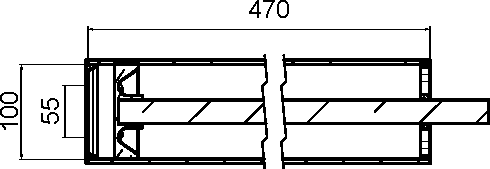
\includegraphics[width=0.8\textwidth]{papers/wirbelringe/fig/zeichnung.pdf}
\caption{Zeichnung und Masse der Wirbelringkanone \cite{Wirbelringe:3D_modelle} \label{Wirbelringe:fig:zeichnung}}
\end{figure}
Für den Bau wird ein (oder Zugang zu einem) 3D Drucker, \diameter 100 PVC Abflussrohr und eine Möglichkeit, Rauch zu erzeugen, um die Wirbelringe besser zu sehen. 
Es müssen lediglich alle Teile 3D gedruckt werden (siehe \cite{Wirbelringe:3D_modelle}) und diese mit einem PVC Kleber fixiert werden. 
Die Konstruktion ist in Abbildung \ref{buch:papers:Wirbelringe:fig:zeichnung} dargestellt.

\subsection{Versuch}

Diese Wirbelringkanone kann nun verwendet werden, um einen Versuch durchzuführen. 
Aus Abschnitt \ref{paper:Wirbelringe:Grenzflaechen} ist bekannt, das Wirbel nur auf Grenzflächen oder sich selbst enden können. 
Um das bei einem Wirbelring aufzuzeigen, kann ein Wirbelring "gespalten" werden. 
Also ein Wirbelring soll dazu gebracht werden, die Grenzflächen von sich selbst auf etwas anderes zu ändern, zum Beispiel ein Tisch. 
Mithilfe einer Kante, die wie eine Klinge funktioniert, kann der Wirbelring geschnitten werden und so umgelenkt, dass der jetzige Wirbelfaden sich weiter bewegt. 
Dieser Versuch ist in Abbildung \ref{buch:papers:Wirbelringe:fig:wirbelringversuch} dargestellt.

\begin{figure}
    \centering
    \subfigure[\label{Wirbelringe:fig:versuch_moment_1}]{
        %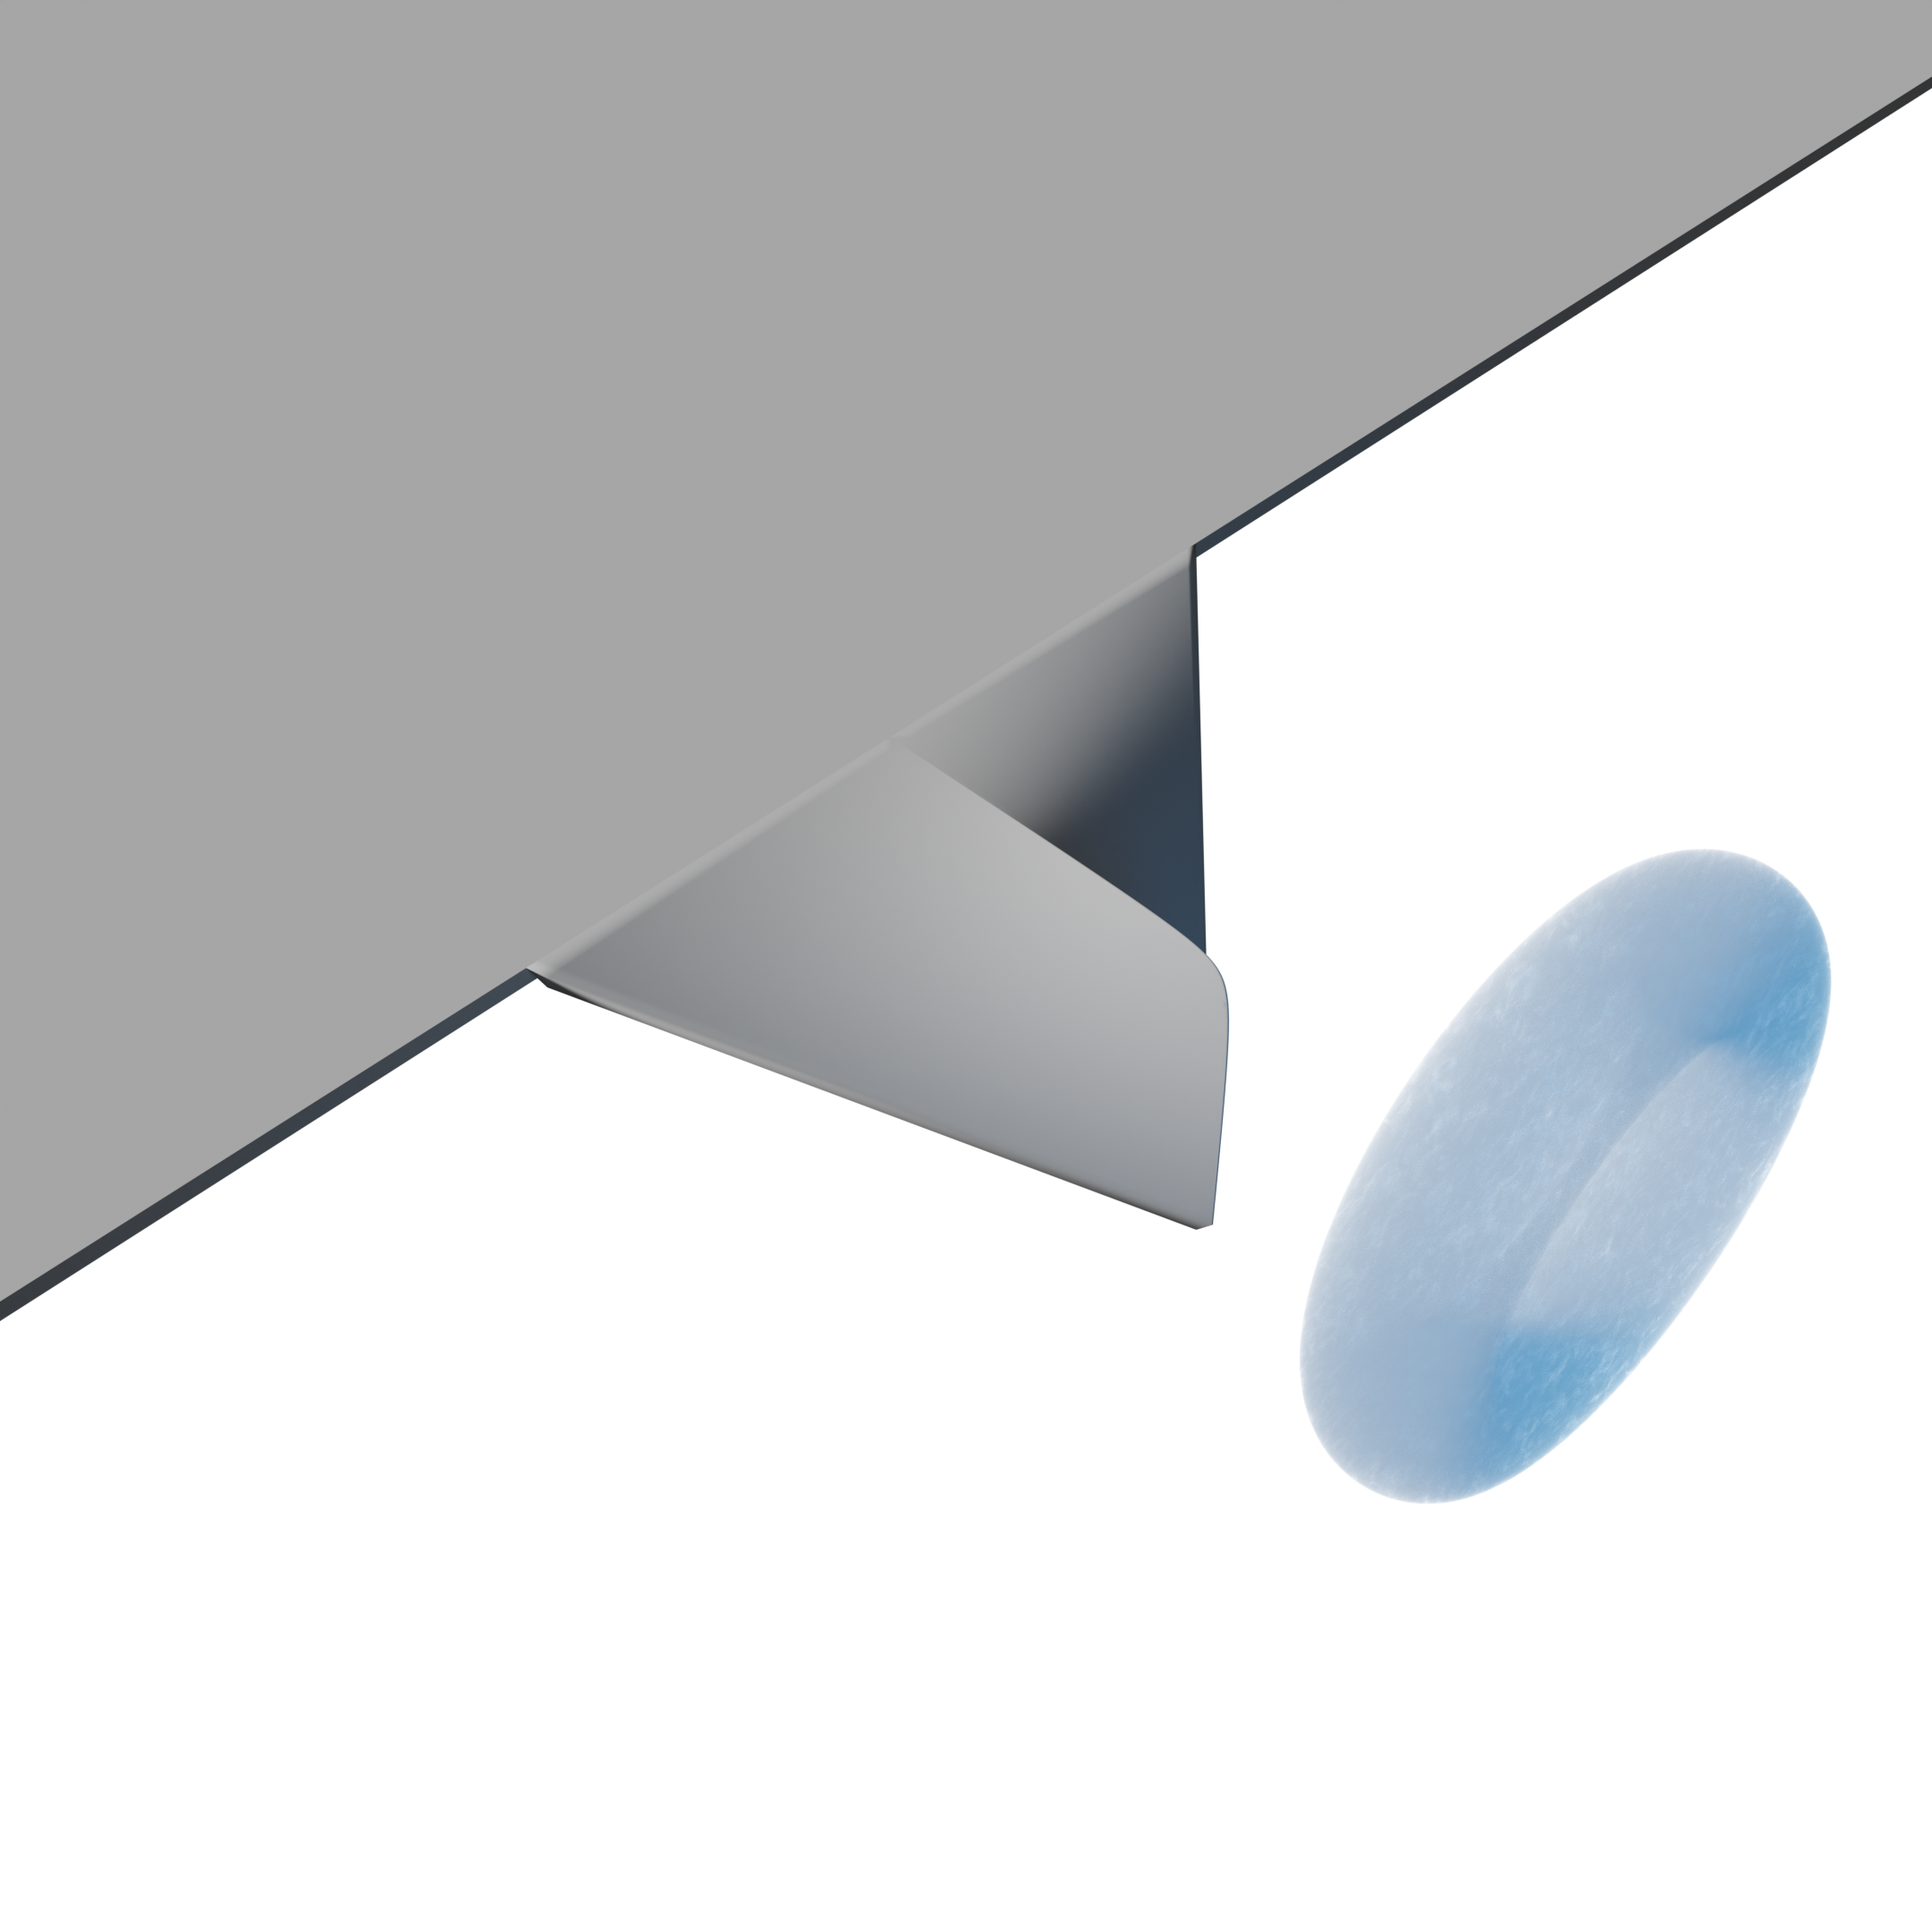
\includegraphics[width=0.3\textwidth]{papers/wirbelringe/fig/versuch_moment_1.png}
        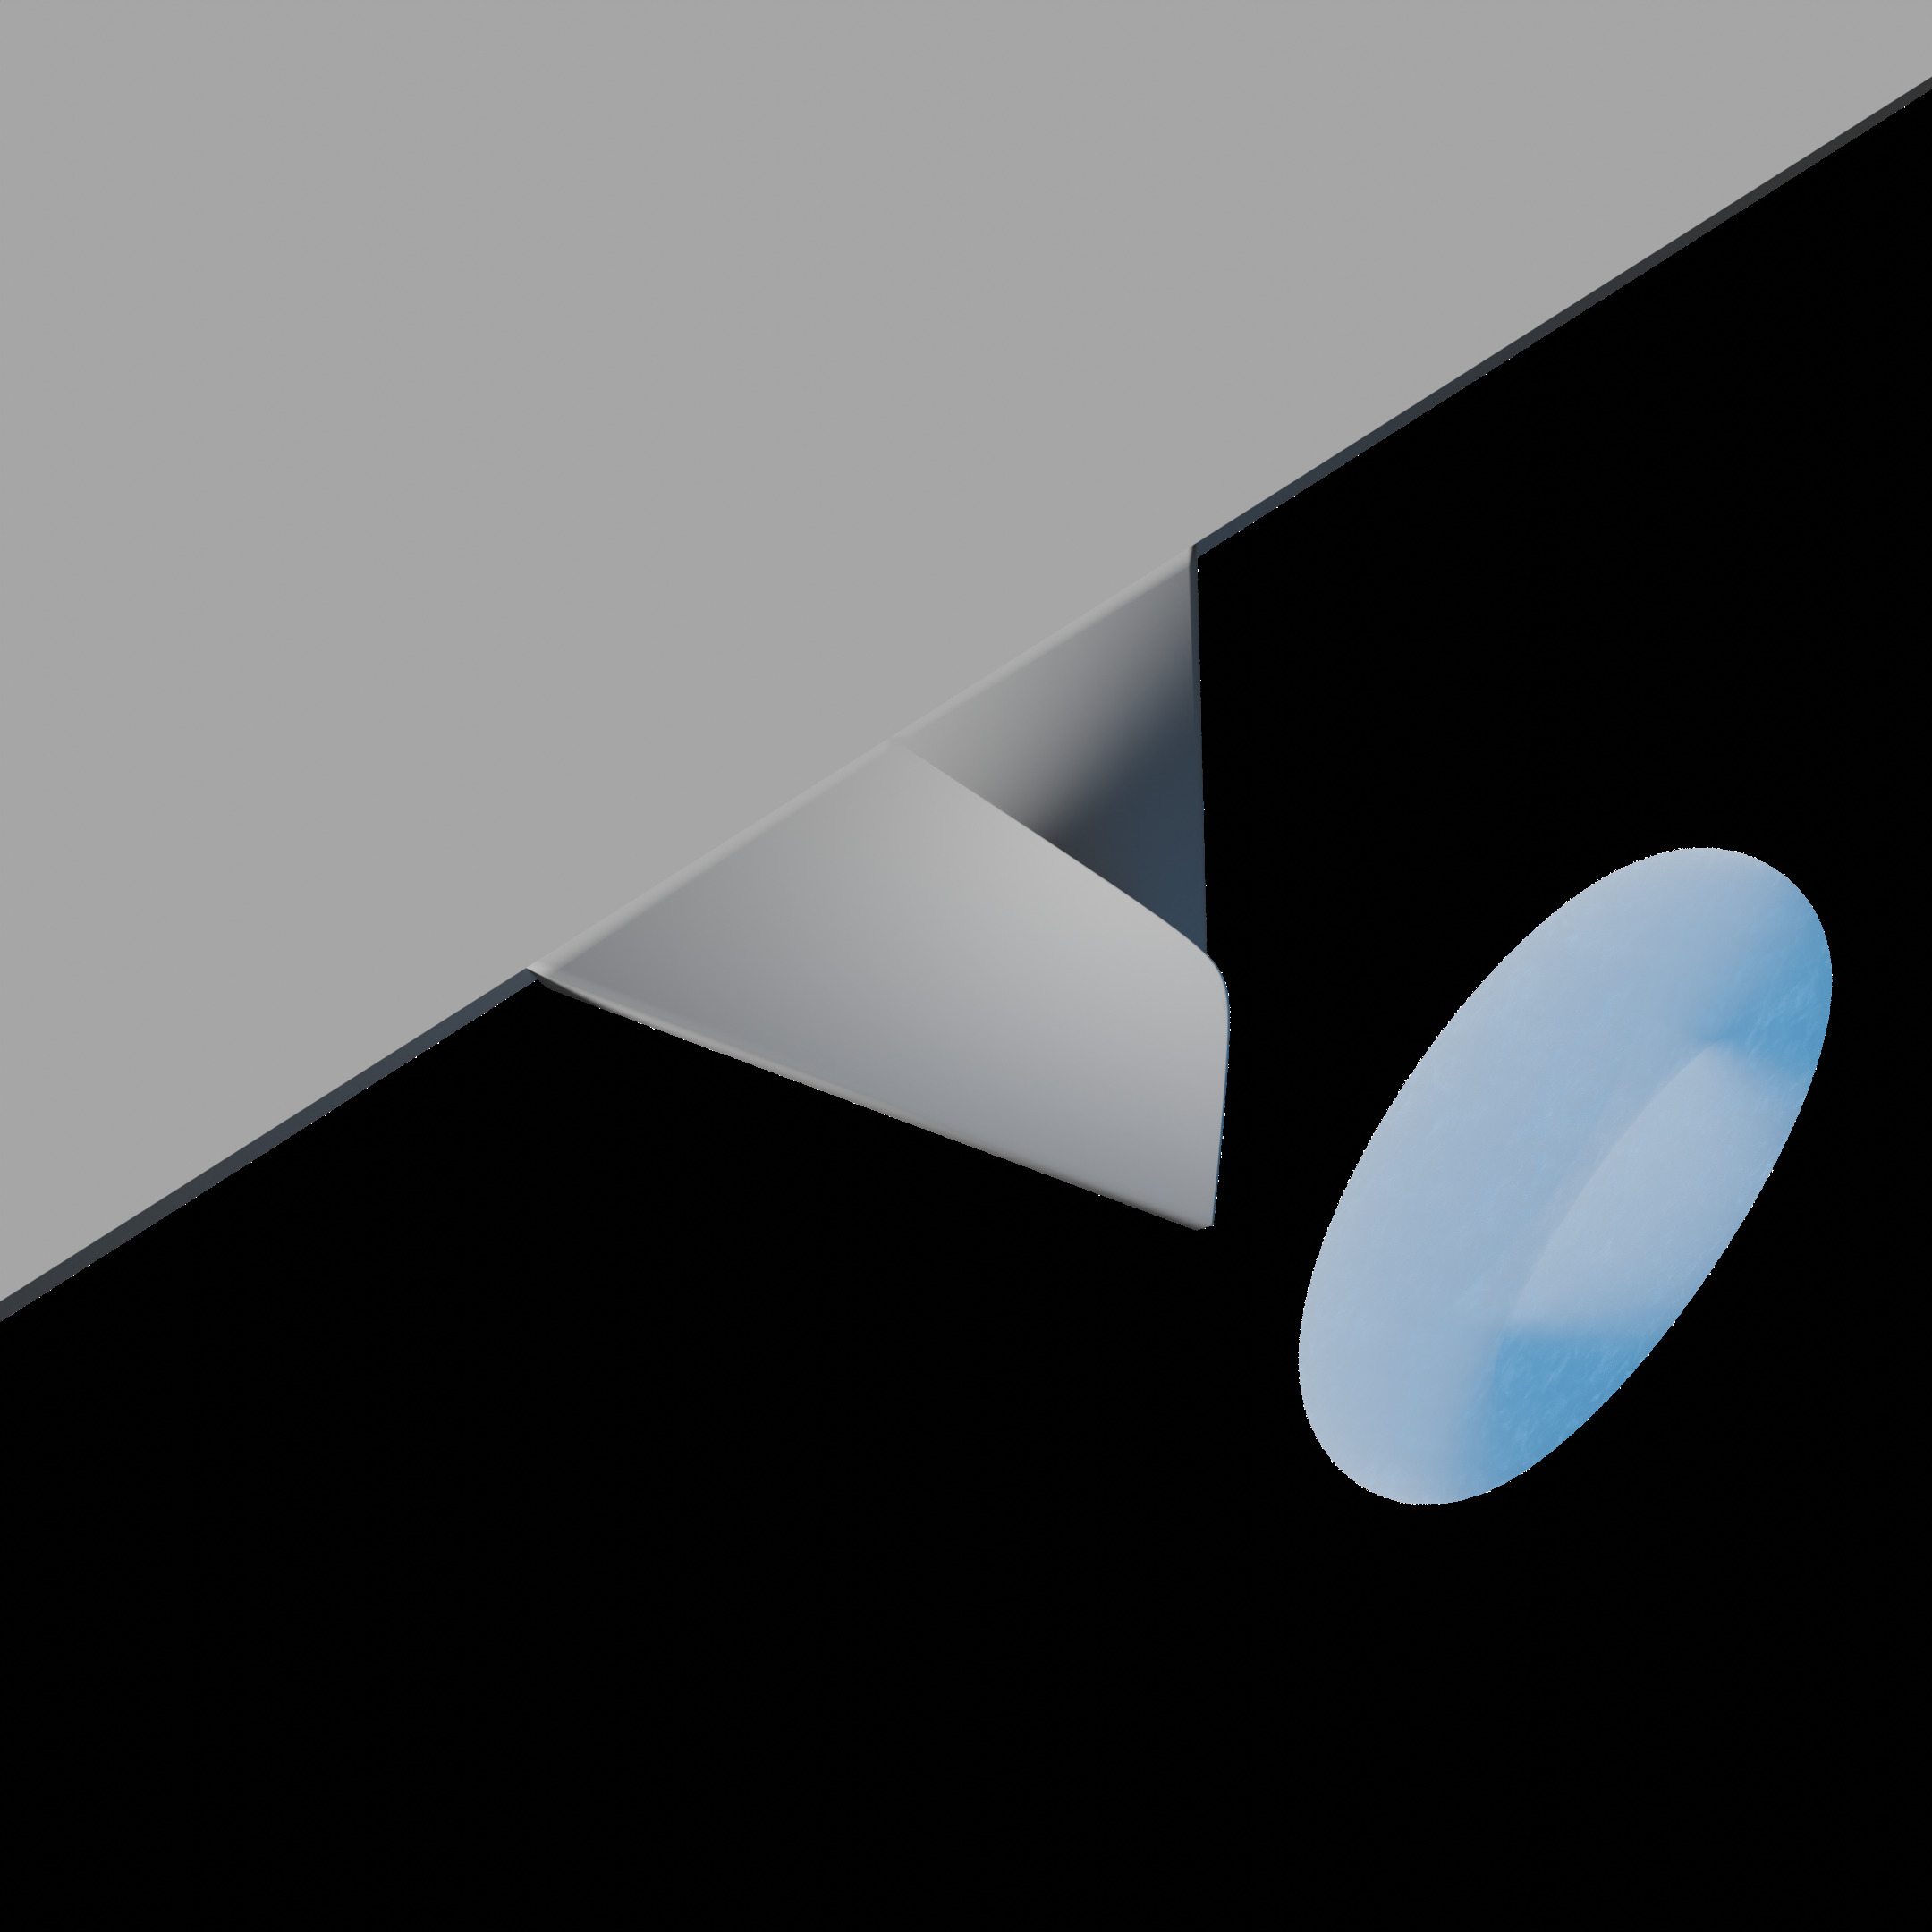
\includegraphics[width=0.3\textwidth]{papers/wirbelringe/fig/versuch_moment_1.jpg}
    }\hfill
    \subfigure[\label{Wirbelringe:fig:versuch_moment_2}]{
        %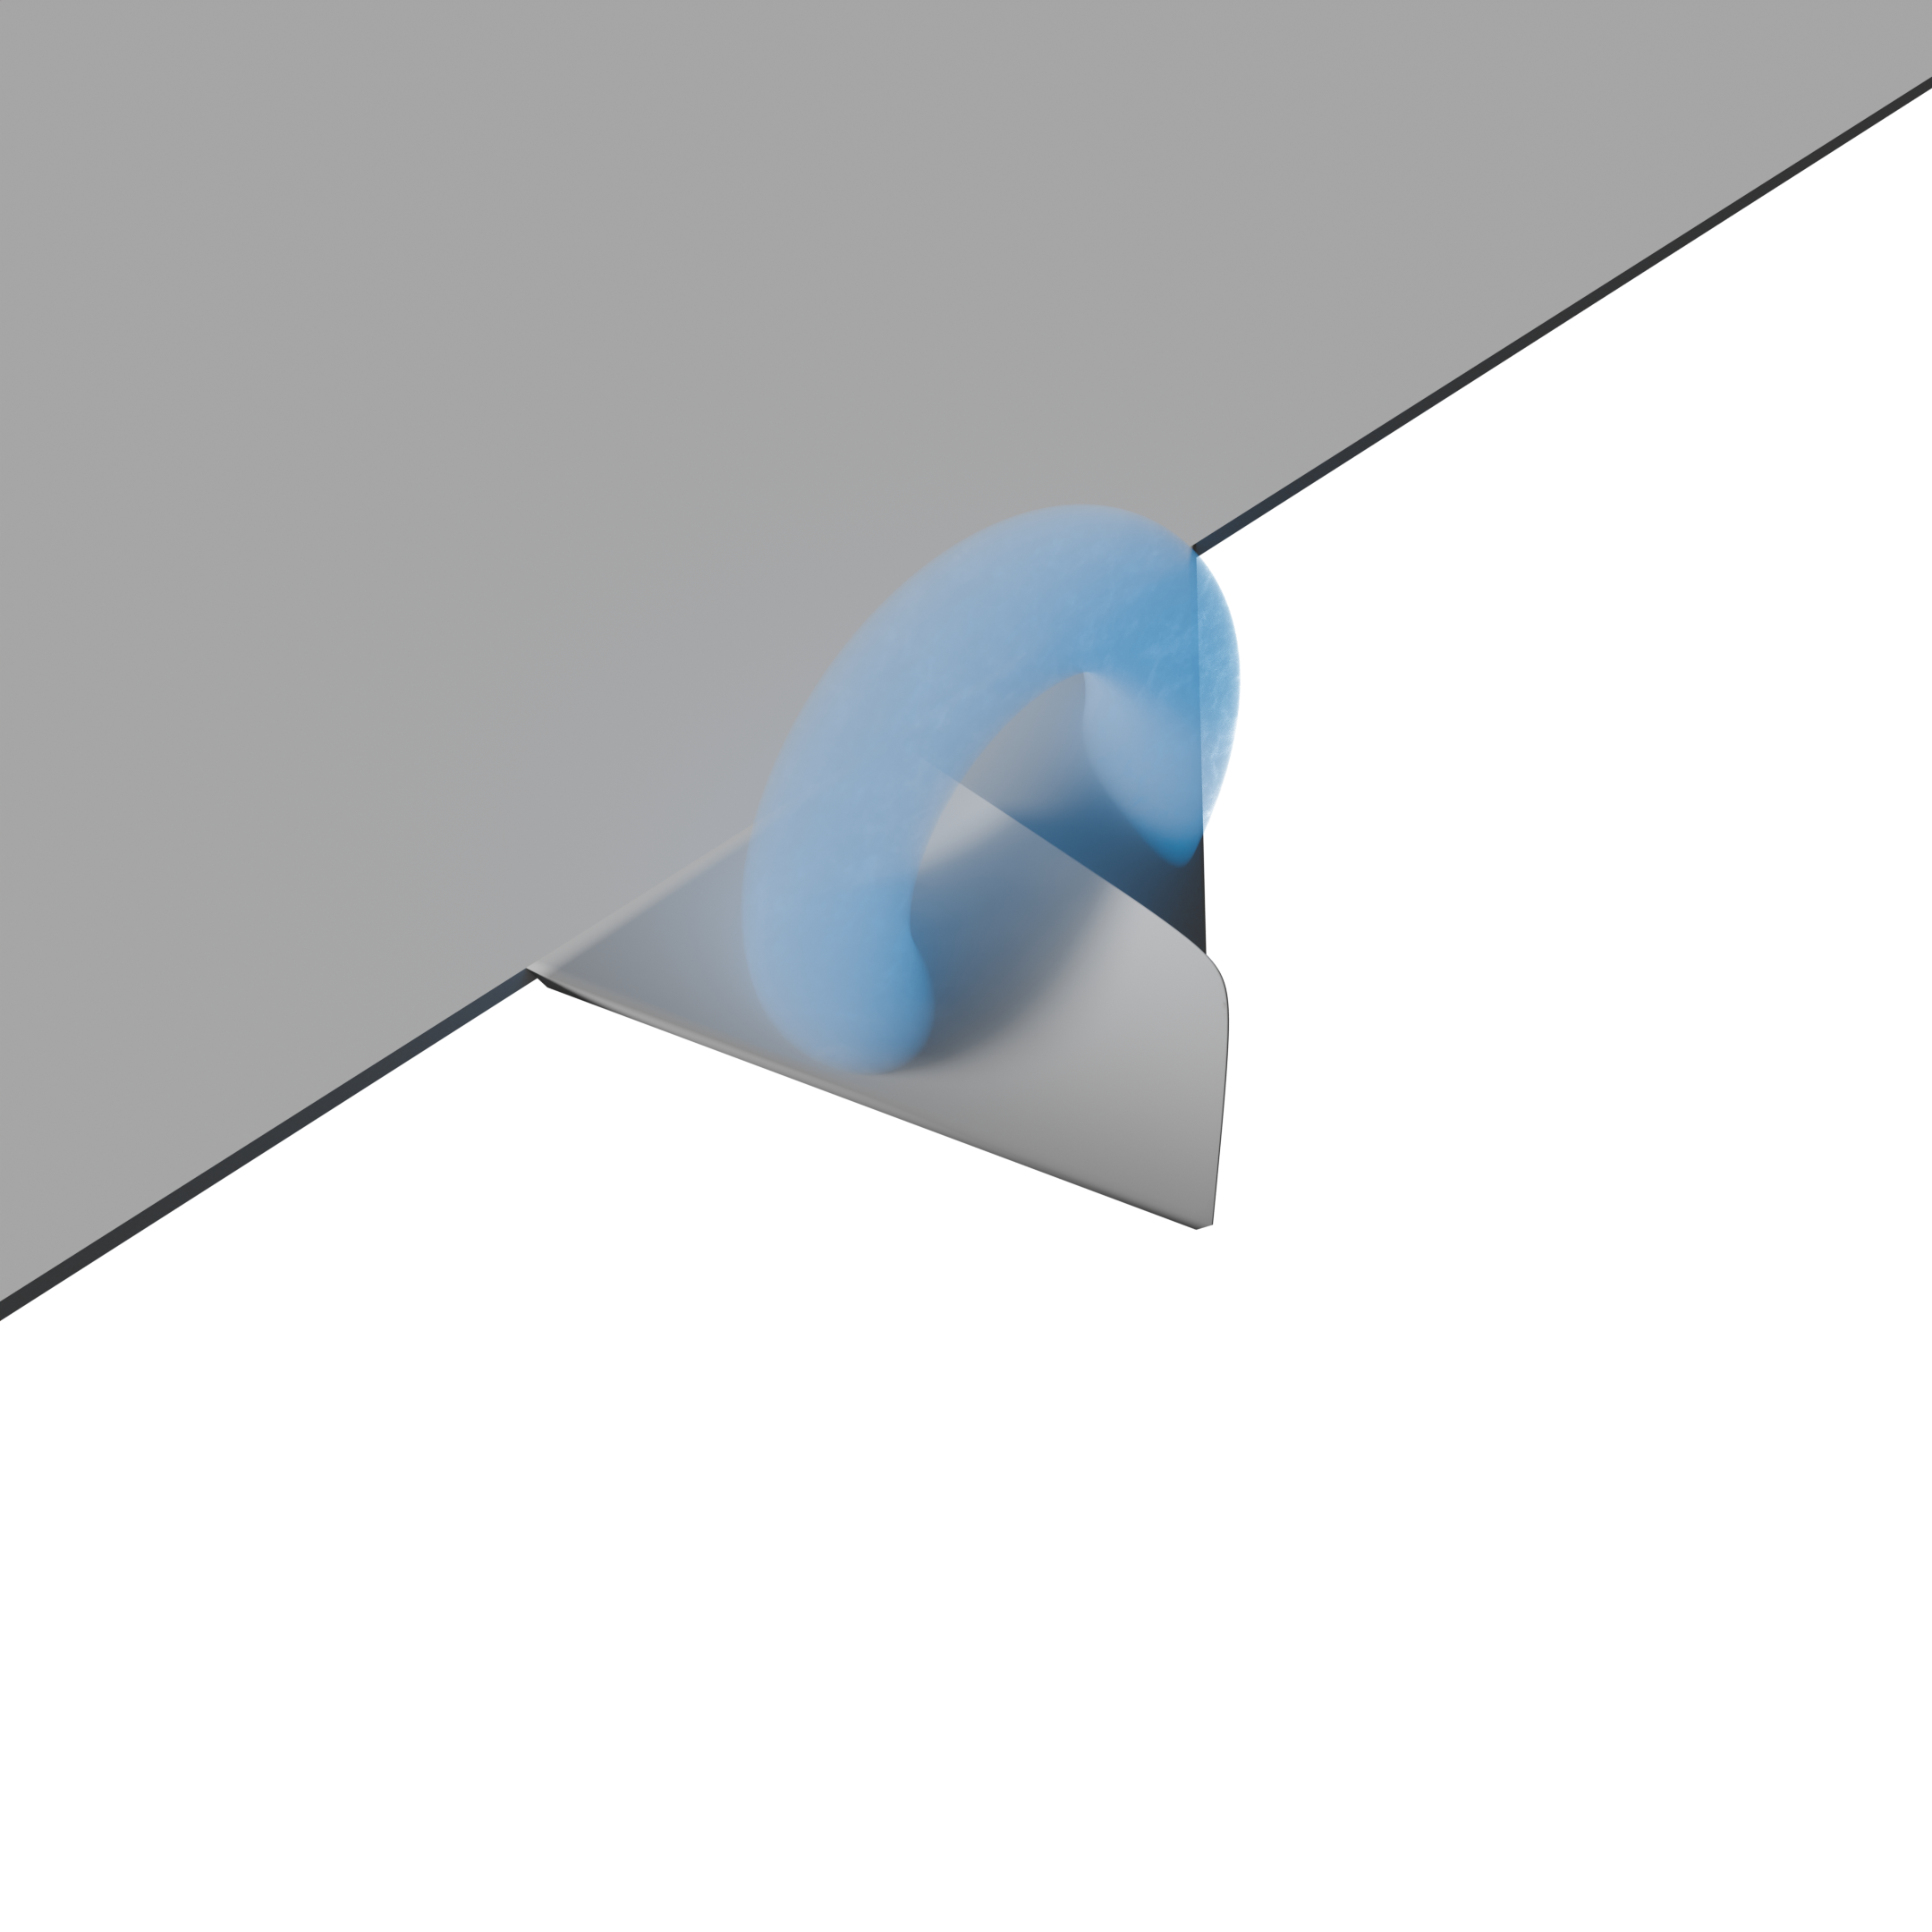
\includegraphics[width=0.3\textwidth]{papers/wirbelringe/fig/versuch_moment_2.png}
        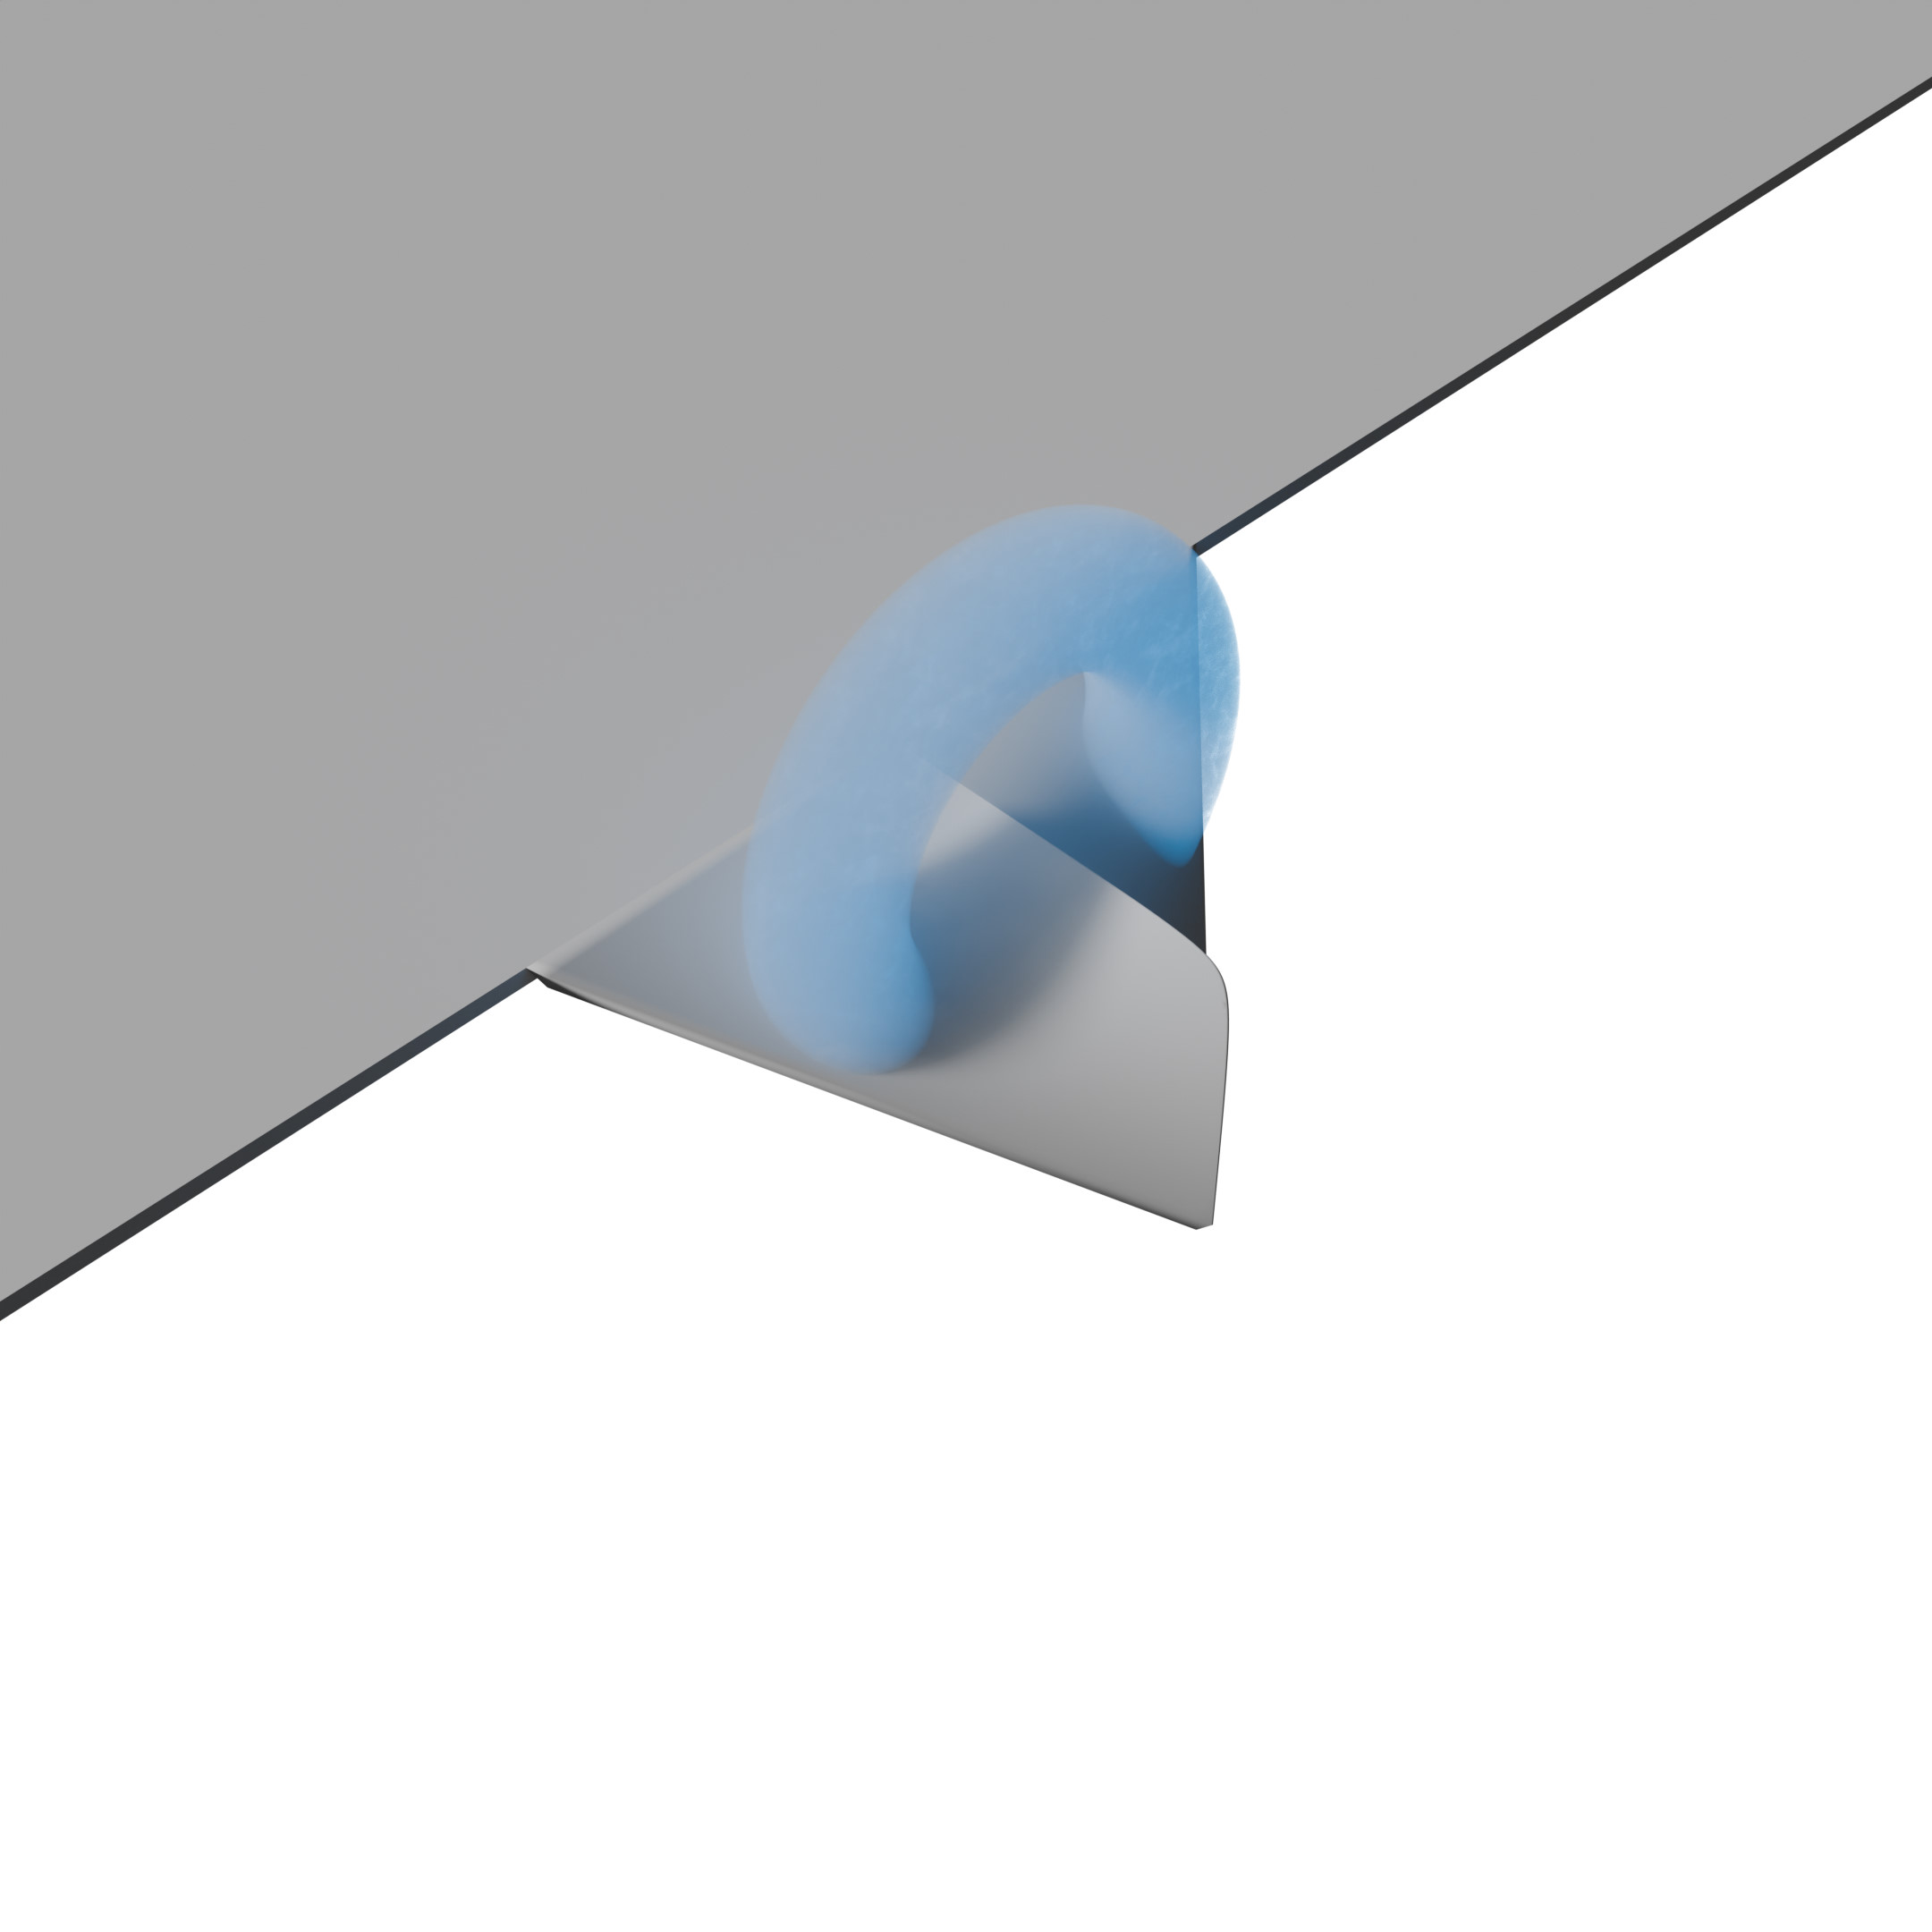
\includegraphics[width=0.3\textwidth]{papers/wirbelringe/fig/versuch_moment_2.jpg}
    }\hfill
    \subfigure[\label{Wirbelringe:fig:versuch_moment_3}]{
        %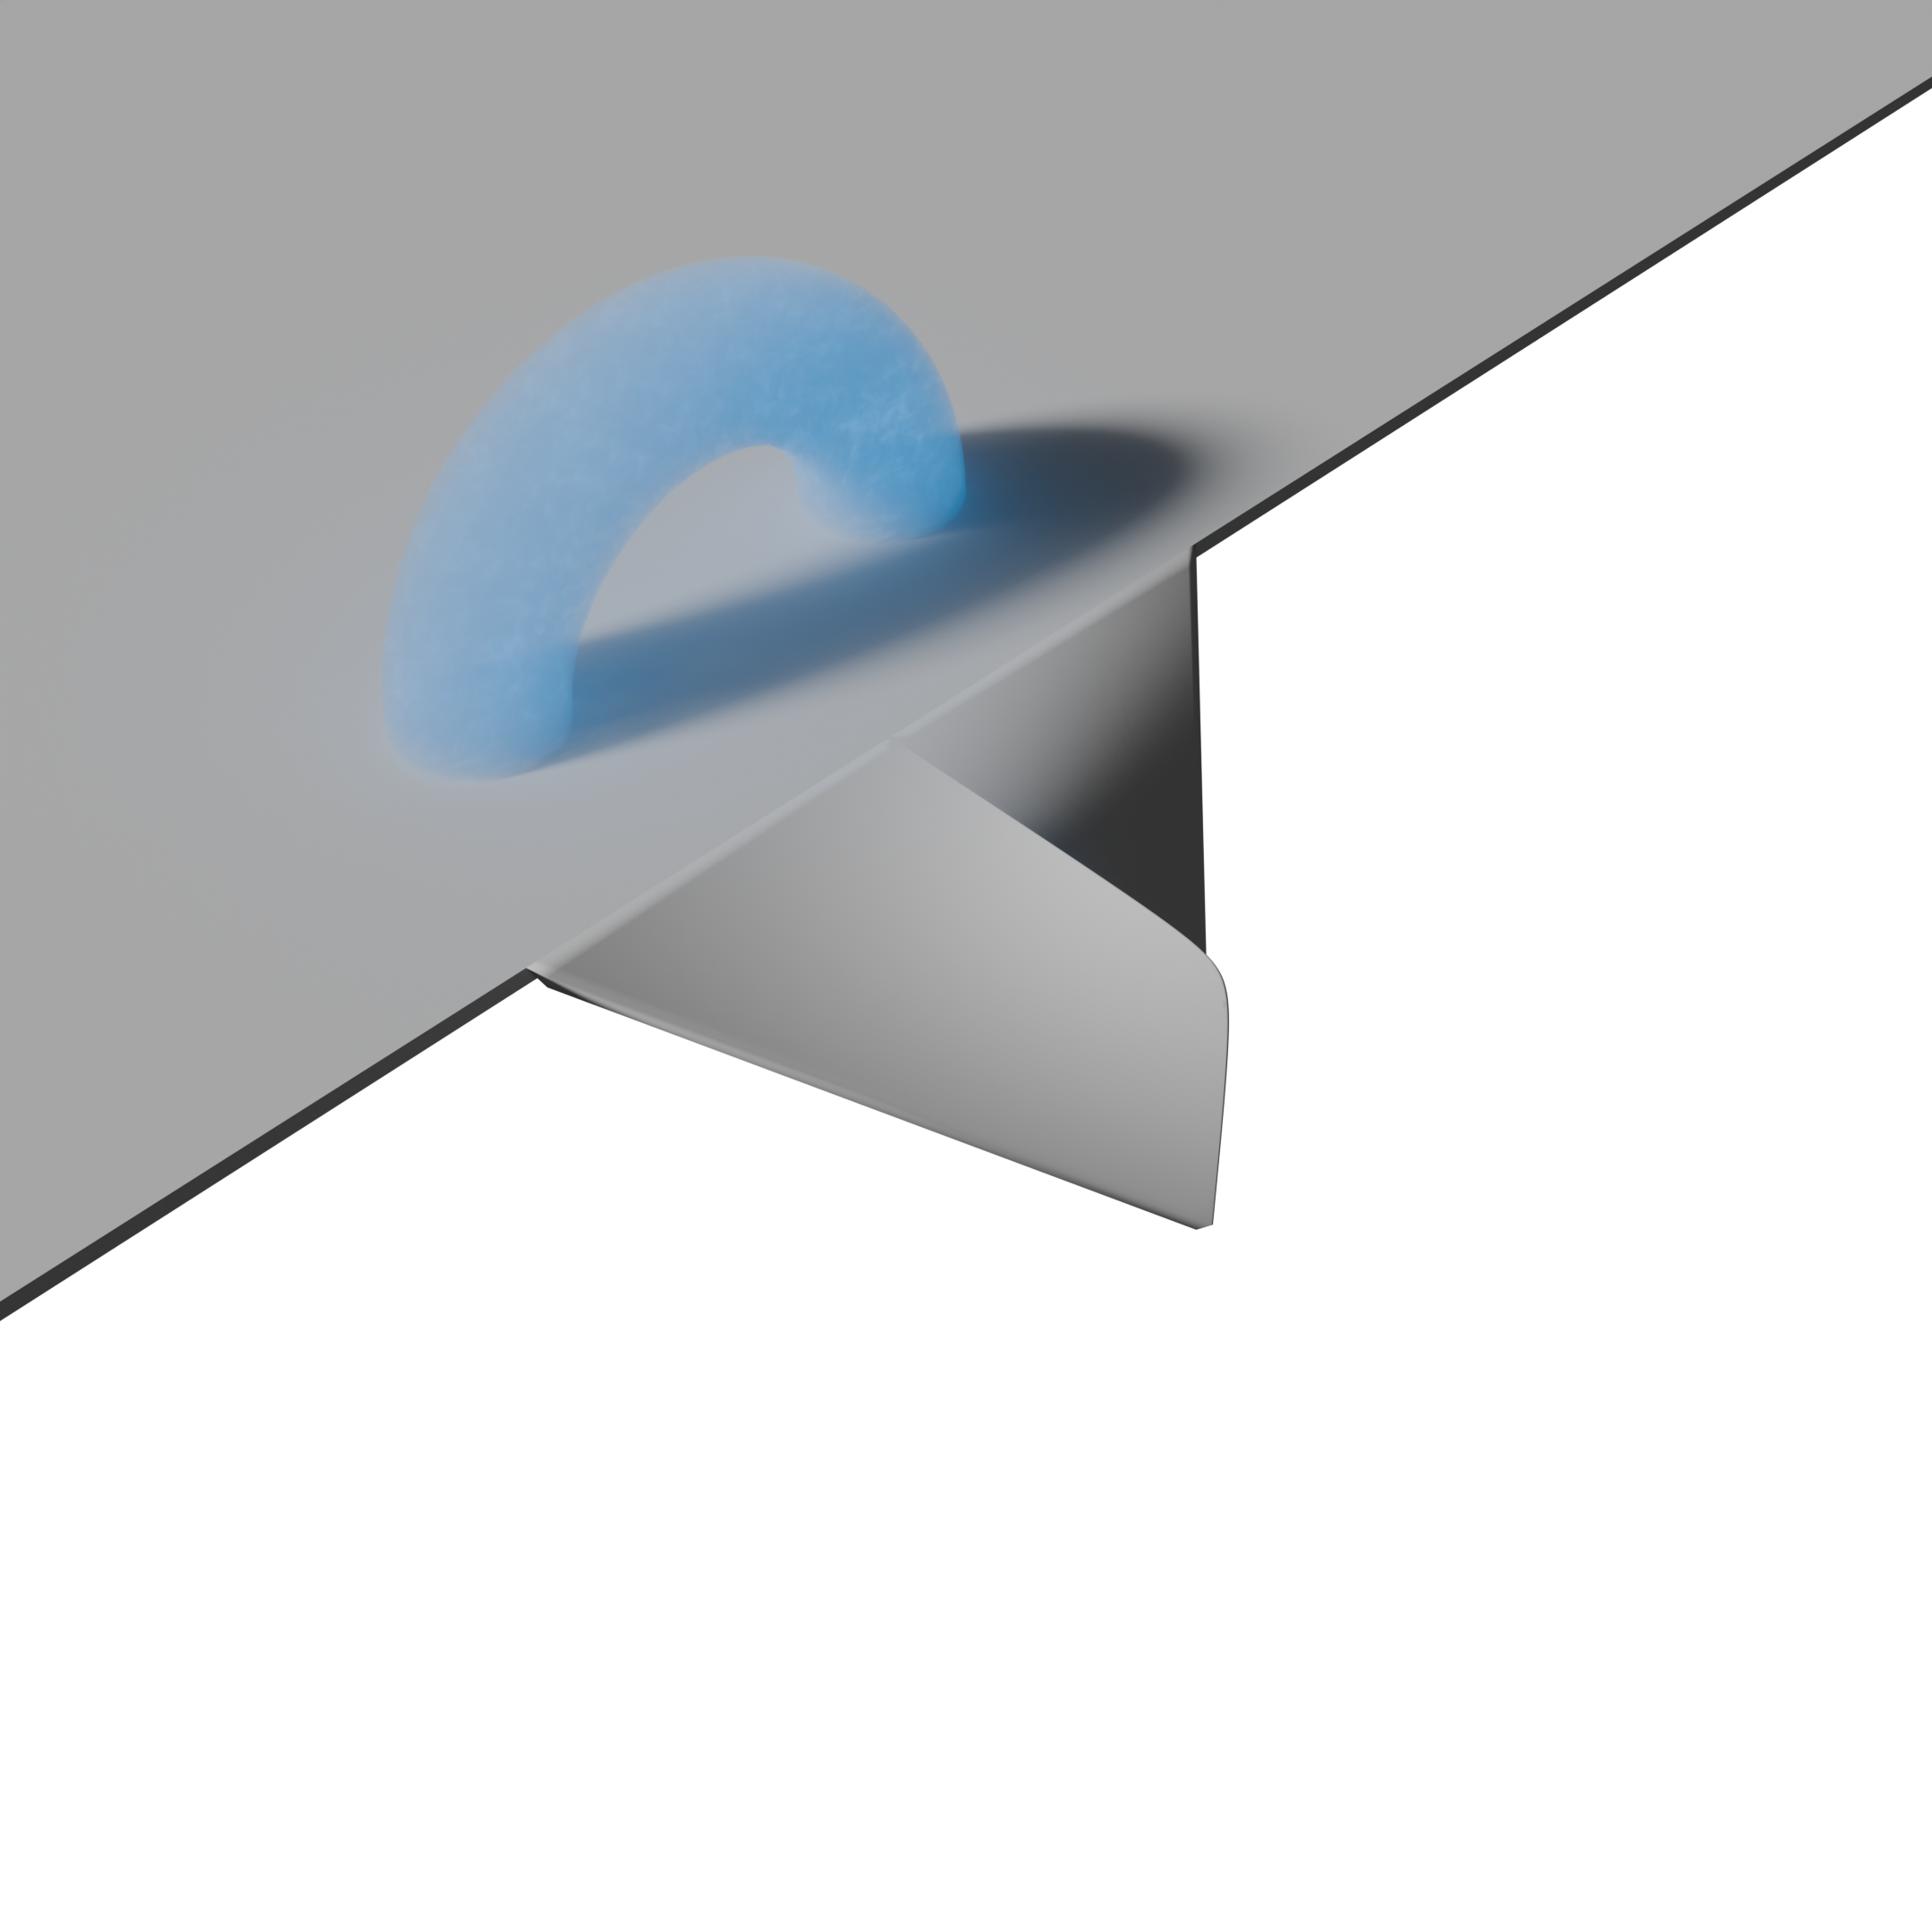
\includegraphics[width=0.3\textwidth]{papers/wirbelringe/fig/versuch_moment_3.png}
        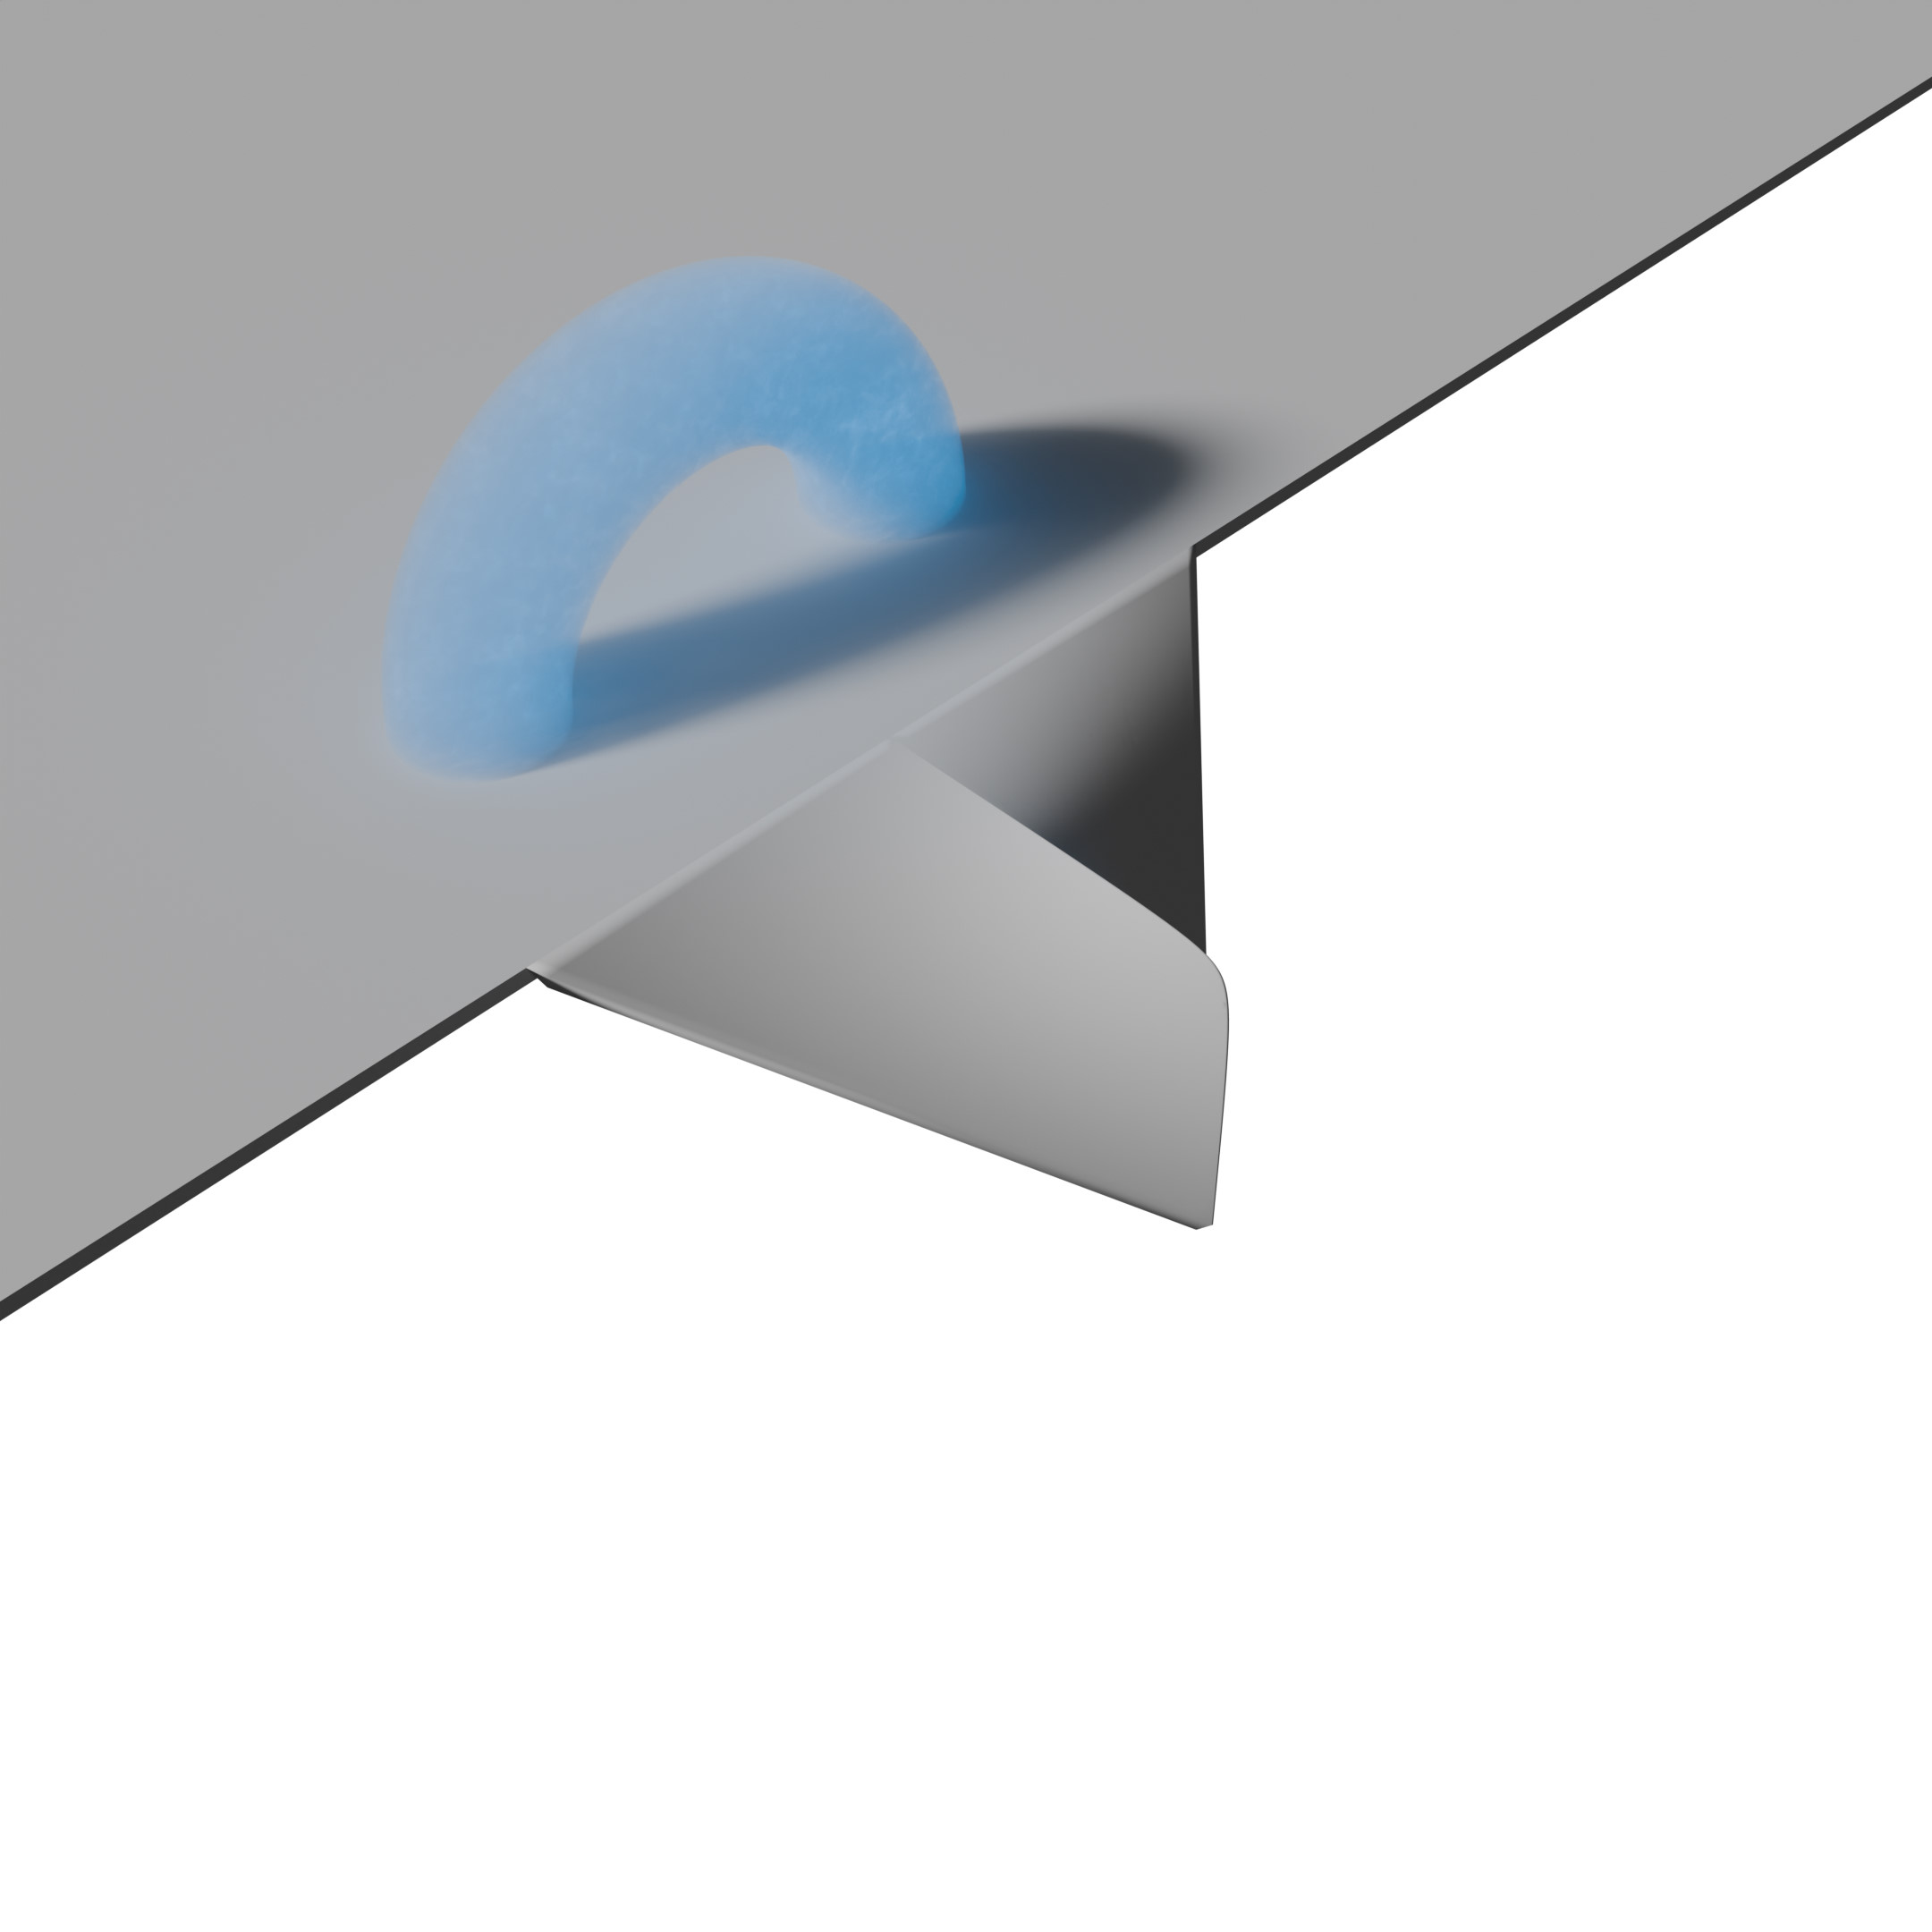
\includegraphics[width=0.3\textwidth]{papers/wirbelringe/fig/versuch_moment_3.jpg}
    }
    \caption{3D Darstellung in Blender des gewünschten Versuchsausgangs.}
    \label{Wirbelringe:fig:wirbelringversuch}
\end{figure}



\printbibliography[heading=subbibliography]
\end{refsection}
